% =====================================================================
%  QAOA for MaxCut — a scaling study
%  BBL540E Graduate Quantum Algorithms course presentation, İTÜ
%  Build: ./build.sh   (runs pdflatex twice for TOC/refs)
% =====================================================================
\documentclass[aspectratio=169,10pt]{beamer}

% ---------- theme ----------
\usetheme{metropolis}
\usecolortheme{default}
\setbeamercolor{frametitle}{bg=black!92!white, fg=white}
\setbeamercolor{progress bar}{fg=qaoablue}
\setbeamercolor{title separator}{fg=qaoablue}
\setbeamercolor{alerted text}{fg=qaoablue}

% ---------- packages ----------
\usepackage[utf8]{inputenc}
\usepackage[T1]{fontenc}
\usepackage{amsmath, amssymb, amsthm}
\usepackage{braket}
\usepackage{graphicx}
\usepackage{booktabs}
\usepackage{tikz}
\usetikzlibrary{arrows.meta, positioning, shapes.geometric, calc}
\usepackage{xcolor}

% ---------- palette matches results/figures colours ----------
\definecolor{qaoablue}{HTML}{2E86AB}     % p=1
\definecolor{qaoapurple}{HTML}{A23B72}   % p=2
\definecolor{qaoaorange}{HTML}{F18F01}   % p=3
\definecolor{lightgrey}{HTML}{888888}

% ---------- math shortcuts ----------
\newcommand{\HC}{H_{C}}
\newcommand{\HB}{H_{B}}
\newcommand{\UC}{U_{C}(\gamma)}
\newcommand{\UB}{U_{B}(\beta)}
\newcommand{\Cstar}{C^{\ast}}
\newcommand{\hz}[1]{\ket{#1}}
\newcommand{\expect}[1]{\langle #1 \rangle}
\newcommand{\one}{\mathbb{1}}

% ---------- figure path ----------
\graphicspath{{../results/figures/}}

% ---------- metadata ----------
\title{QAOA for MaxCut}
\subtitle{A scaling study on 3-regular graphs}
\author{Özgün Can Yürütken \\ \footnotesize Student ID: 707251003}
\institute{BBL540E — Quantum Data Structures \& Algorithms \\
           \footnotesize Instructor: Doç.\ Dr.\ Deniz Türkpençe \\
           İstanbul Technical University}
\date{April 2026}

\begin{document}

% ---------------------------------------------------------------------
\begin{frame}[plain]
  \titlepage
\end{frame}

% ---------------------------------------------------------------------
\begin{frame}{MaxCut — the classical problem}
  \begin{columns}[T,onlytextwidth]
    \begin{column}{0.55\textwidth}
      Given an unweighted, undirected graph $G = (V, E)$, find a partition
      $S \subseteq V$ that maximises the number of \emph{crossing} edges:
      \[
        C(S) = \bigl|\{(u,v)\in E : u\in S,\, v\notin S\}\bigr|,
      \]
      \[
        \Cstar = \max_{S \subseteq V} C(S).
      \]
      \vspace{0.2em}
      \textbf{Why it is a good benchmark}
      \begin{itemize}
        \item NP-hard; no efficient classical exact algorithm known.
        \item Best classical approximation: Goemans–Williamson,
              ratio $\approx 0.878$ (1995).
        \item NISQ-friendly: graph is sparse, Hamiltonian is diagonal,
              circuit depth scales gently.
      \end{itemize}
    \end{column}
    \begin{column}{0.42\textwidth}
      \centering
      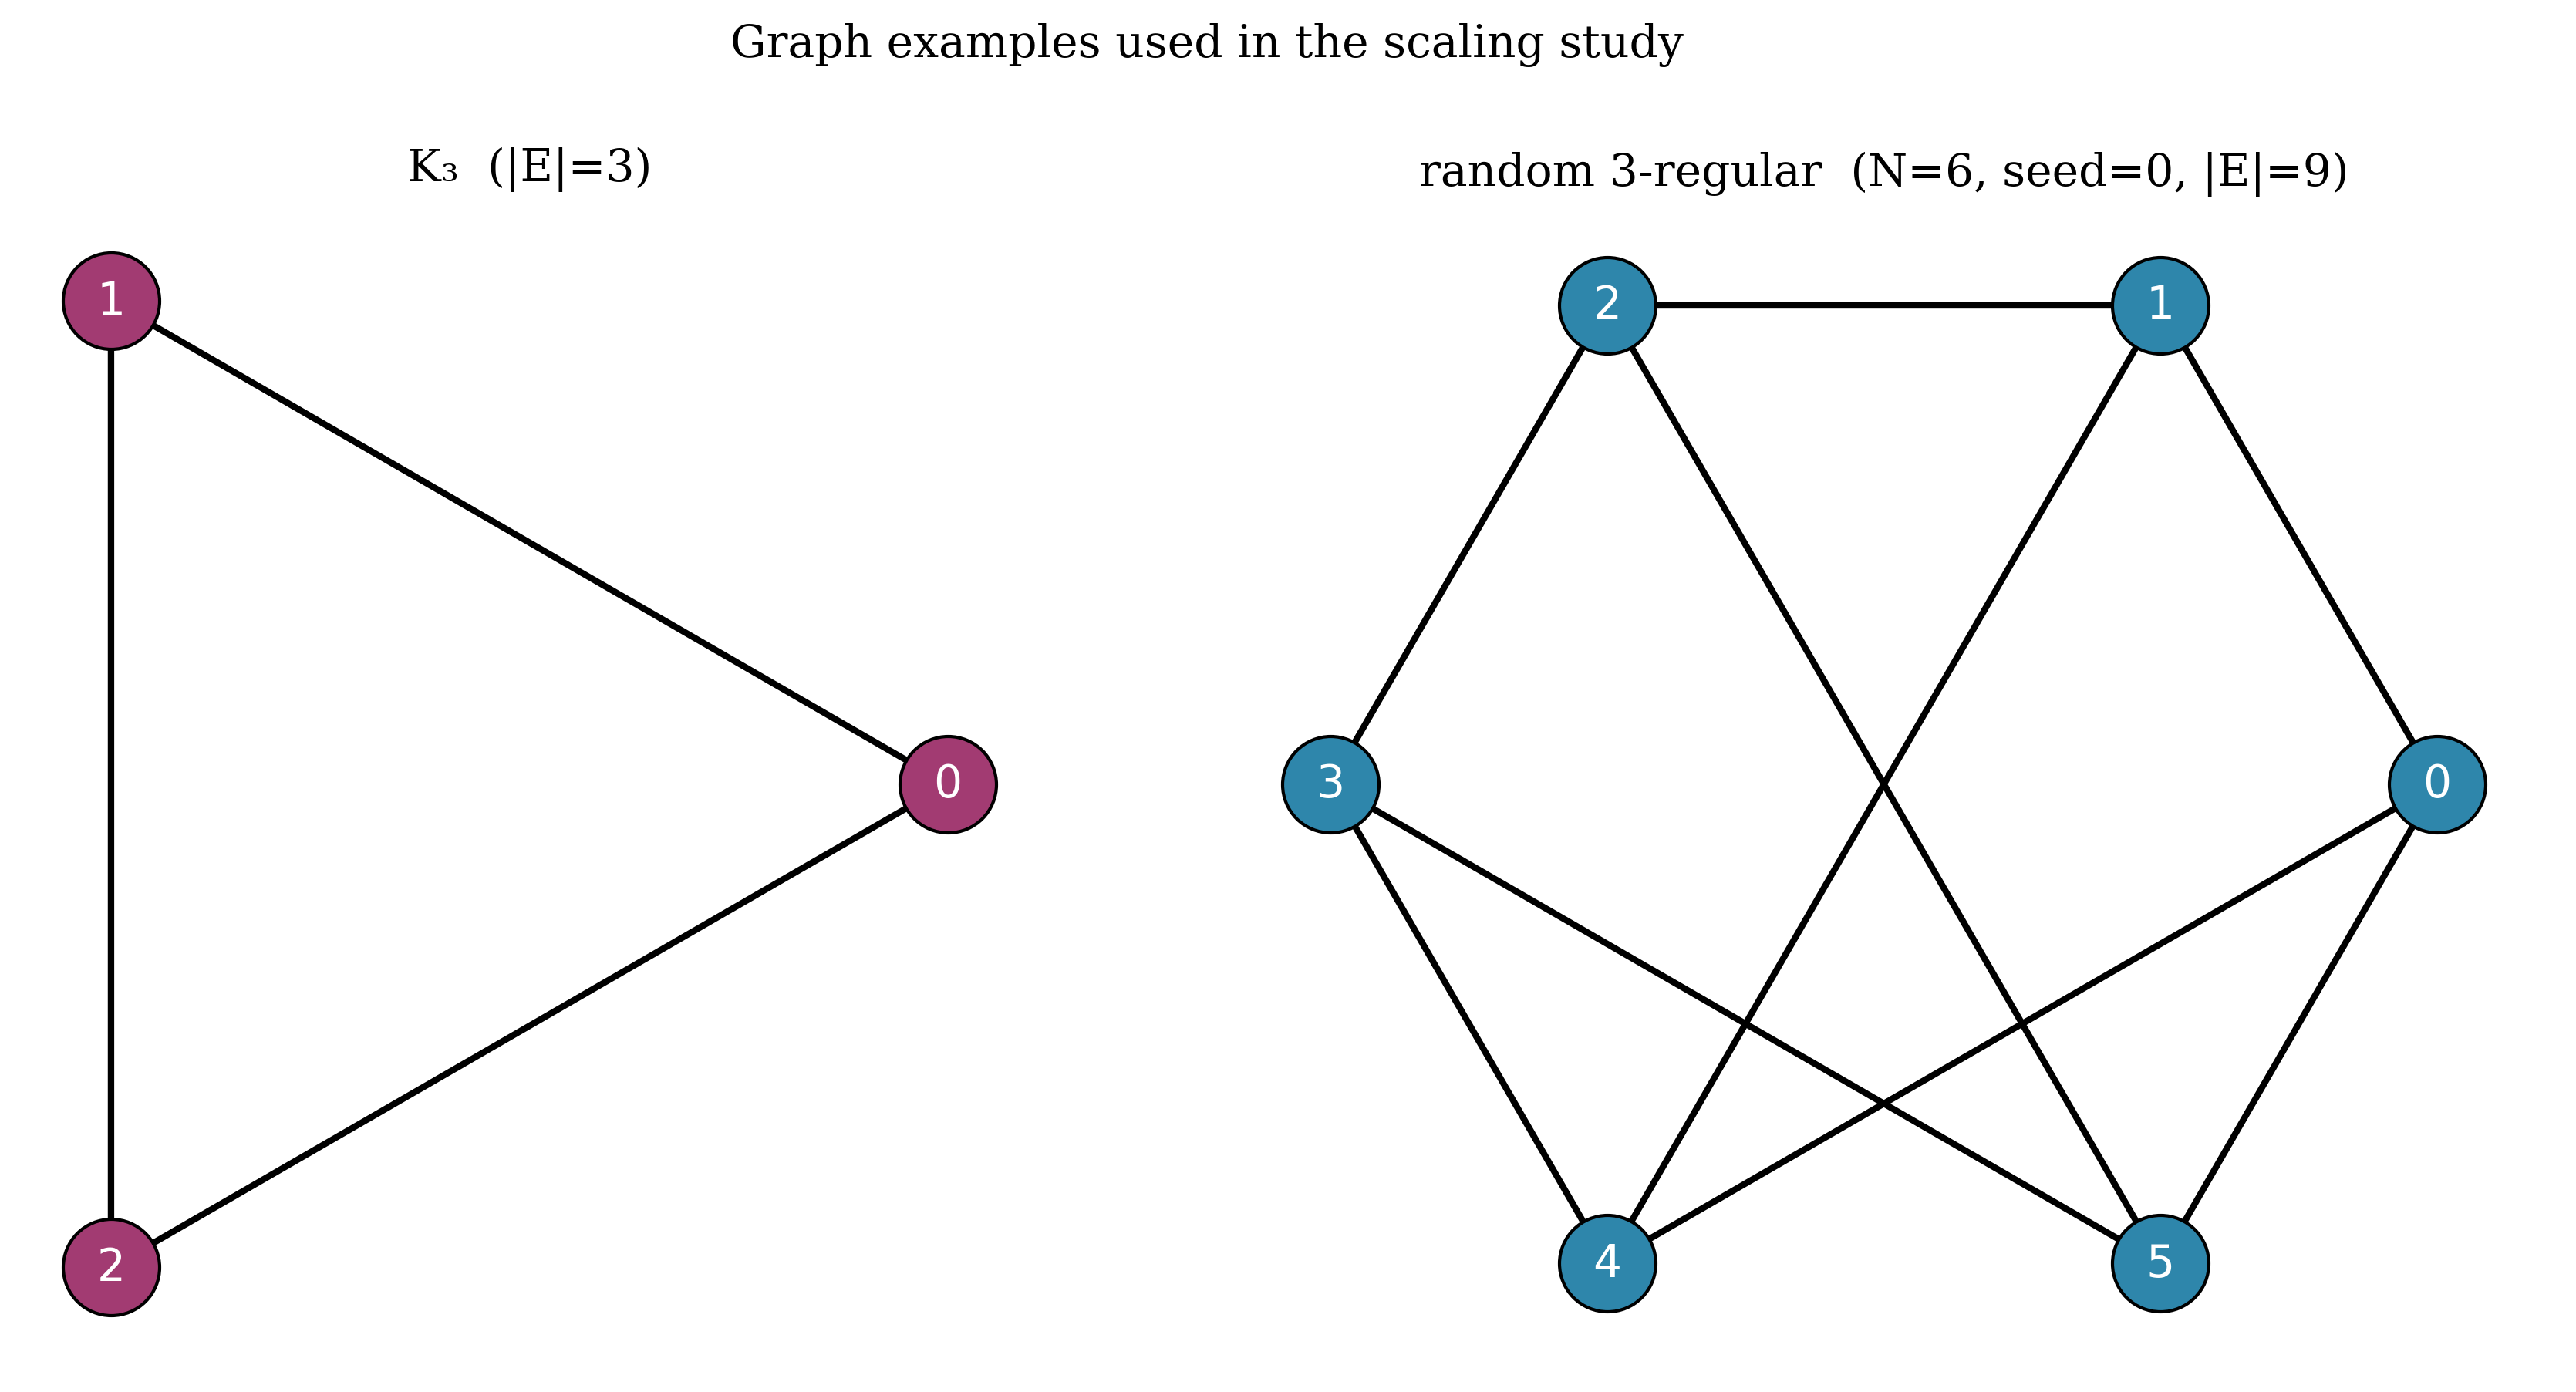
\includegraphics[width=\linewidth]{09_graph_examples.png}
      \\[-0.2em]
      {\scriptsize Two representative instances from this study.}
    \end{column}
  \end{columns}
\end{frame}

% ---------------------------------------------------------------------
\begin{frame}{From bits to spins — the Ising encoding}
  \begin{columns}[T,onlytextwidth]
    \begin{column}{0.52\textwidth}
      \small
      Binary $x_i\in\{0,1\}$, spin $s_i = 1-2x_i \in \{\pm1\}$
      (so $x_i{=}0\Leftrightarrow i\in S$).
      Substituting $x_i=(1-s_i)/2$ in the cut objective and promoting
      $s_i \to Z_i$:
      \[
        \boxed{\;\HC \;=\; \tfrac{1}{2}\sum_{(i,j)\in E}\bigl(Z_i Z_j - \one\bigr)\;}
      \]
      Every computational basis state is an eigenstate:
      $\HC \hz{z} = -C(z)\,\hz{z}$ — the \alert{ground state is the
      optimal cut}.
    \end{column}
    \begin{column}{0.44\textwidth}
      \textbf{K$_3$ spectrum (our toy problem)}
      \vspace{0.3em}
      \begin{center}
      \scriptsize
      \begin{tabular}{cccc}
        \toprule
        eigenvalue & mult.\ & $C(z)$ & states \\
        \midrule
        $-2$ & $6$ & $2$ & cuts \\
        $\phantom{-}0$ & $2$ & $0$ & $\hz{000},\hz{111}$ \\
        \bottomrule
      \end{tabular}
      \end{center}
      \vspace{0.3em}
      \small Uniform baseline (K$_3$):
      $\bra{\psi_0}\HC\ket{\psi_0} = -\tfrac{3}{2},\ r=0.75$.
      Any non-trivial quantum algorithm must beat this.
    \end{column}
  \end{columns}
  \vspace{0.3em}
  \scriptsize\color{gray}
  Convention: $\HC$ minimisation form (Qiskit-compatible); Farhi~2014
  uses the opposite sign.
\end{frame}

% ---------------------------------------------------------------------
\begin{frame}{The QAOA ansatz}
  \[
    \ket{\psi_p(\boldsymbol{\gamma},\boldsymbol{\beta})}
      \;=\;
      U_B(\beta_p)\,U_C(\gamma_p)\,\cdots\,U_B(\beta_1)\,U_C(\gamma_1)\;
      H^{\otimes n}\ket{0}^{\otimes n}.
  \]
  \begin{columns}[T,onlytextwidth]
    \begin{column}{0.48\textwidth}
      \small\textbf{Cost operator}
      \[
        \UC \;=\; \prod_{(i,j)\in E} e^{-i\frac{\gamma}{2} Z_i Z_j}
      \]
      Per edge, $R_z(\theta)=e^{-i\frac{\theta}{2}\sigma_z}$:
      \[
        e^{-i\frac{\gamma}{2}Z_iZ_j} =
        \text{CX}_{i,j}\,R_z(\gamma)_j\,\text{CX}_{i,j}
      \]
      $\Rightarrow 2|E|$ CNOTs per layer.
    \end{column}
    \begin{column}{0.48\textwidth}
      \small\textbf{Mixer operator}
      \[
        \UB \;=\; \prod_{i=0}^{n-1} e^{-i\beta X_i}
            \;=\; \prod_{i} R_x(2\beta)_i
      \]
      $R_x(\theta)=e^{-i\frac{\theta}{2}\sigma_x}$ gives the factor
      $2\beta$.\\[0.2em]
      $\Rightarrow n$ single-qubit gates, all parallel (depth 1).
    \end{column}
  \end{columns}
  \vspace{0.3em}
  \small\textbf{Objective}\quad
  $F_p(\boldsymbol\gamma,\boldsymbol\beta) = \bra{\psi_p}\HC\ket{\psi_p}$
  — classical optimiser minimises, quantum device evaluates.
\end{frame}

% ---------------------------------------------------------------------
\begin{frame}{I/O pipeline and the variational loop}
  \begin{columns}[T,onlytextwidth]
    \begin{column}{0.56\textwidth}
      \centering
      \textbf{\small Data encoding $\to$ measurement}\\[0.4em]
      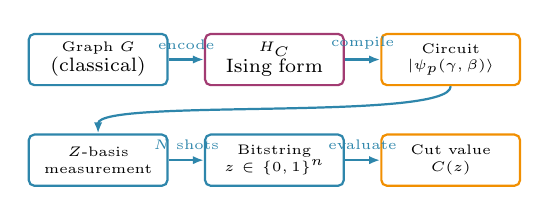
\begin{tikzpicture}[
        node distance=0.45cm,
        every node/.style={font=\tiny},
        box/.style={rectangle, rounded corners=2pt, draw=qaoablue,
                    thick, align=center, inner sep=3pt,
                    minimum height=0.65cm, text width=1.55cm},
        ham/.style={rectangle, rounded corners=2pt, draw=qaoapurple,
                    thick, align=center, inner sep=3pt,
                    minimum height=0.65cm, text width=1.55cm},
        arr/.style={-{Latex[length=1.4mm]}, thick, qaoablue}
      ]
        \node[box] (g) {Graph $G$\\ \scriptsize (classical)};
        \node[ham, right=of g] (h) {$H_C$\\ \scriptsize Ising form};
        \node[box, right=of h, draw=qaoaorange] (c) {Circuit\\ $\ket{\psi_p(\gamma,\beta)}$};
        \node[box, below=0.6cm of g] (m) {$Z$-basis\\ measurement};
        \node[box, right=of m] (z) {Bitstring\\ $z\in\{0,1\}^n$};
        \node[box, right=of z, draw=qaoaorange] (cz) {Cut value\\ $C(z)$};

        \draw[arr] (g) -- node[above]{encode} (h);
        \draw[arr] (h) -- node[above]{compile} (c);
        \draw[arr] (c.south) .. controls +(0,-0.45) and +(0,0.45) .. (m.north);
        \draw[arr] (m) -- node[above]{$N$ shots} (z);
        \draw[arr] (z) -- node[above]{evaluate} (cz);
      \end{tikzpicture}
      \\[0.4em]
      \scriptsize
      \textbf{Input:} graph $\to$ diagonal Hamiltonian
      $H_C=\tfrac12\sum_{(i,j)\in E}(Z_iZ_j-I)$.\\
      \textbf{Output:} best bitstring $z^\ast$ sampled from
      $|\braket{z|\psi_p}|^2$; report $C(z^\ast)$.
    \end{column}
    \begin{column}{0.42\textwidth}
      \centering
      \textbf{\small Hybrid quantum--classical loop}\\[0.4em]
      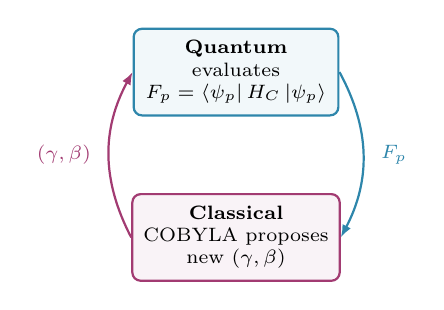
\begin{tikzpicture}[
        every node/.style={font=\scriptsize},
        big/.style={rectangle, rounded corners=3pt, thick, align=center,
                    minimum width=2.6cm, minimum height=1.1cm, inner sep=4pt},
        arr/.style={-{Latex[length=1.6mm]}, thick}
      ]
        \node[big, draw=qaoablue, fill=qaoablue!6] (q) at (0,0)
          {\textbf{Quantum}\\ evaluates\\ $F_p=\bra{\psi_p}\HC\ket{\psi_p}$};
        \node[big, draw=qaoapurple, fill=qaoapurple!6] (c) at (0,-2.1)
          {\textbf{Classical}\\ COBYLA proposes\\ new $(\gamma,\beta)$};
        \draw[arr, qaoablue, bend left=28] (q.east) to
          node[right, xshift=1mm]{$F_p$} (c.east);
        \draw[arr, qaoapurple, bend left=28] (c.west) to
          node[left, xshift=-1mm]{$(\gamma,\beta)$} (q.west);
      \end{tikzpicture}
      \\[0.4em]
      \scriptsize
      Classical side minimises $F_p$; quantum side is only called as a
      black-box expectation oracle.
      \alert{Parameters stay low-dim} ($2p$ floats), so COBYLA
      converges in tens--hundreds of calls.
    \end{column}
  \end{columns}
\end{frame}

% ---------------------------------------------------------------------
\begin{frame}{K$_3$ toy — circuit and parameter landscape}
  \begin{columns}[c,onlytextwidth]
    \begin{column}{0.50\textwidth}
      \centering
      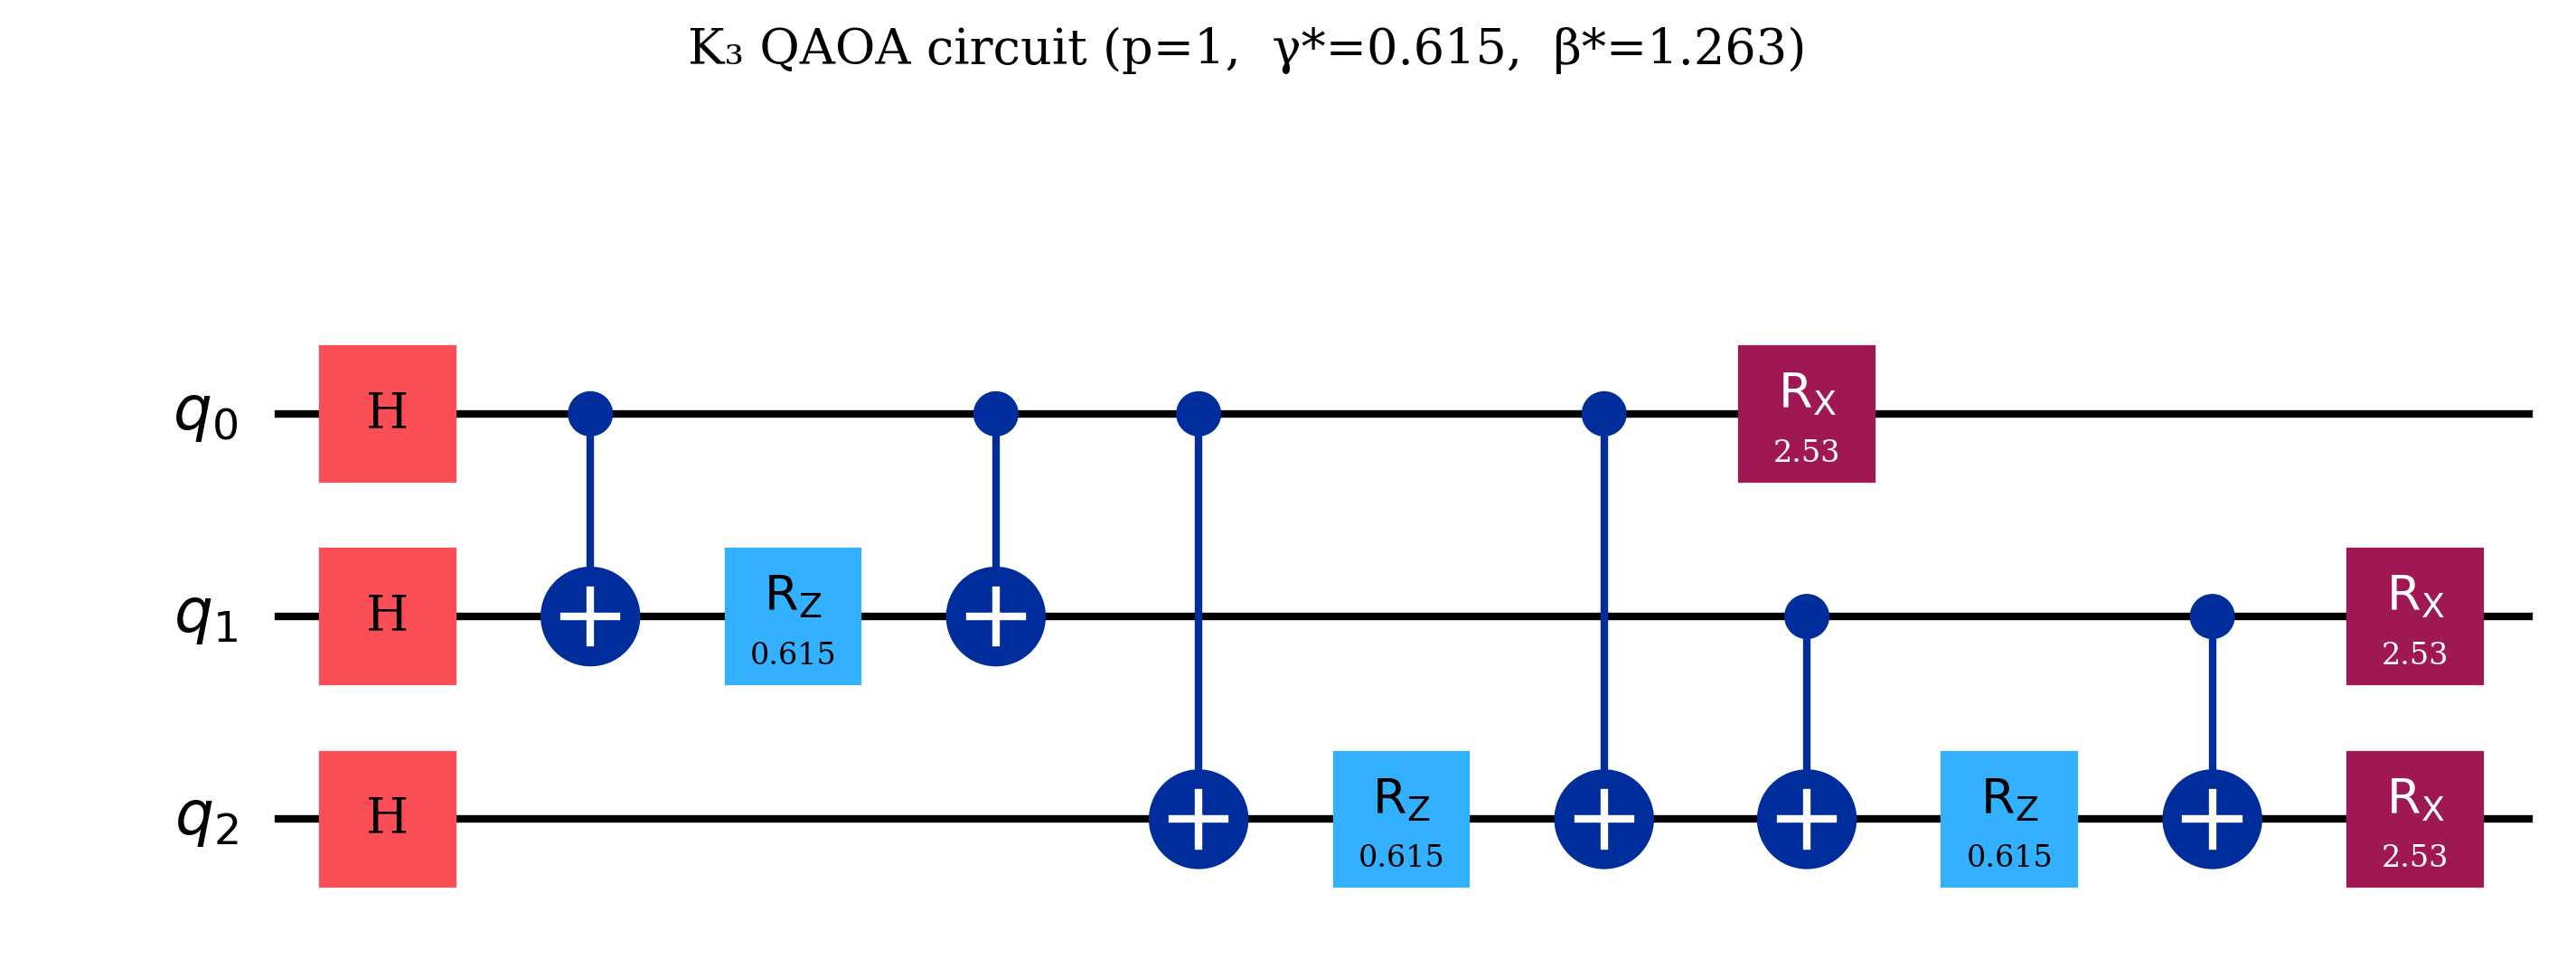
\includegraphics[width=\linewidth]{01_k3_circuit_diagram.png}
      \\[0.2em]
      {\scriptsize $p=1$: $3\,H$ + $3\!\times\!(\text{CX--}R_z\text{--CX})$
         + $3\,R_x(2\beta)$.}
    \end{column}
    \begin{column}{0.48\textwidth}
      \centering
      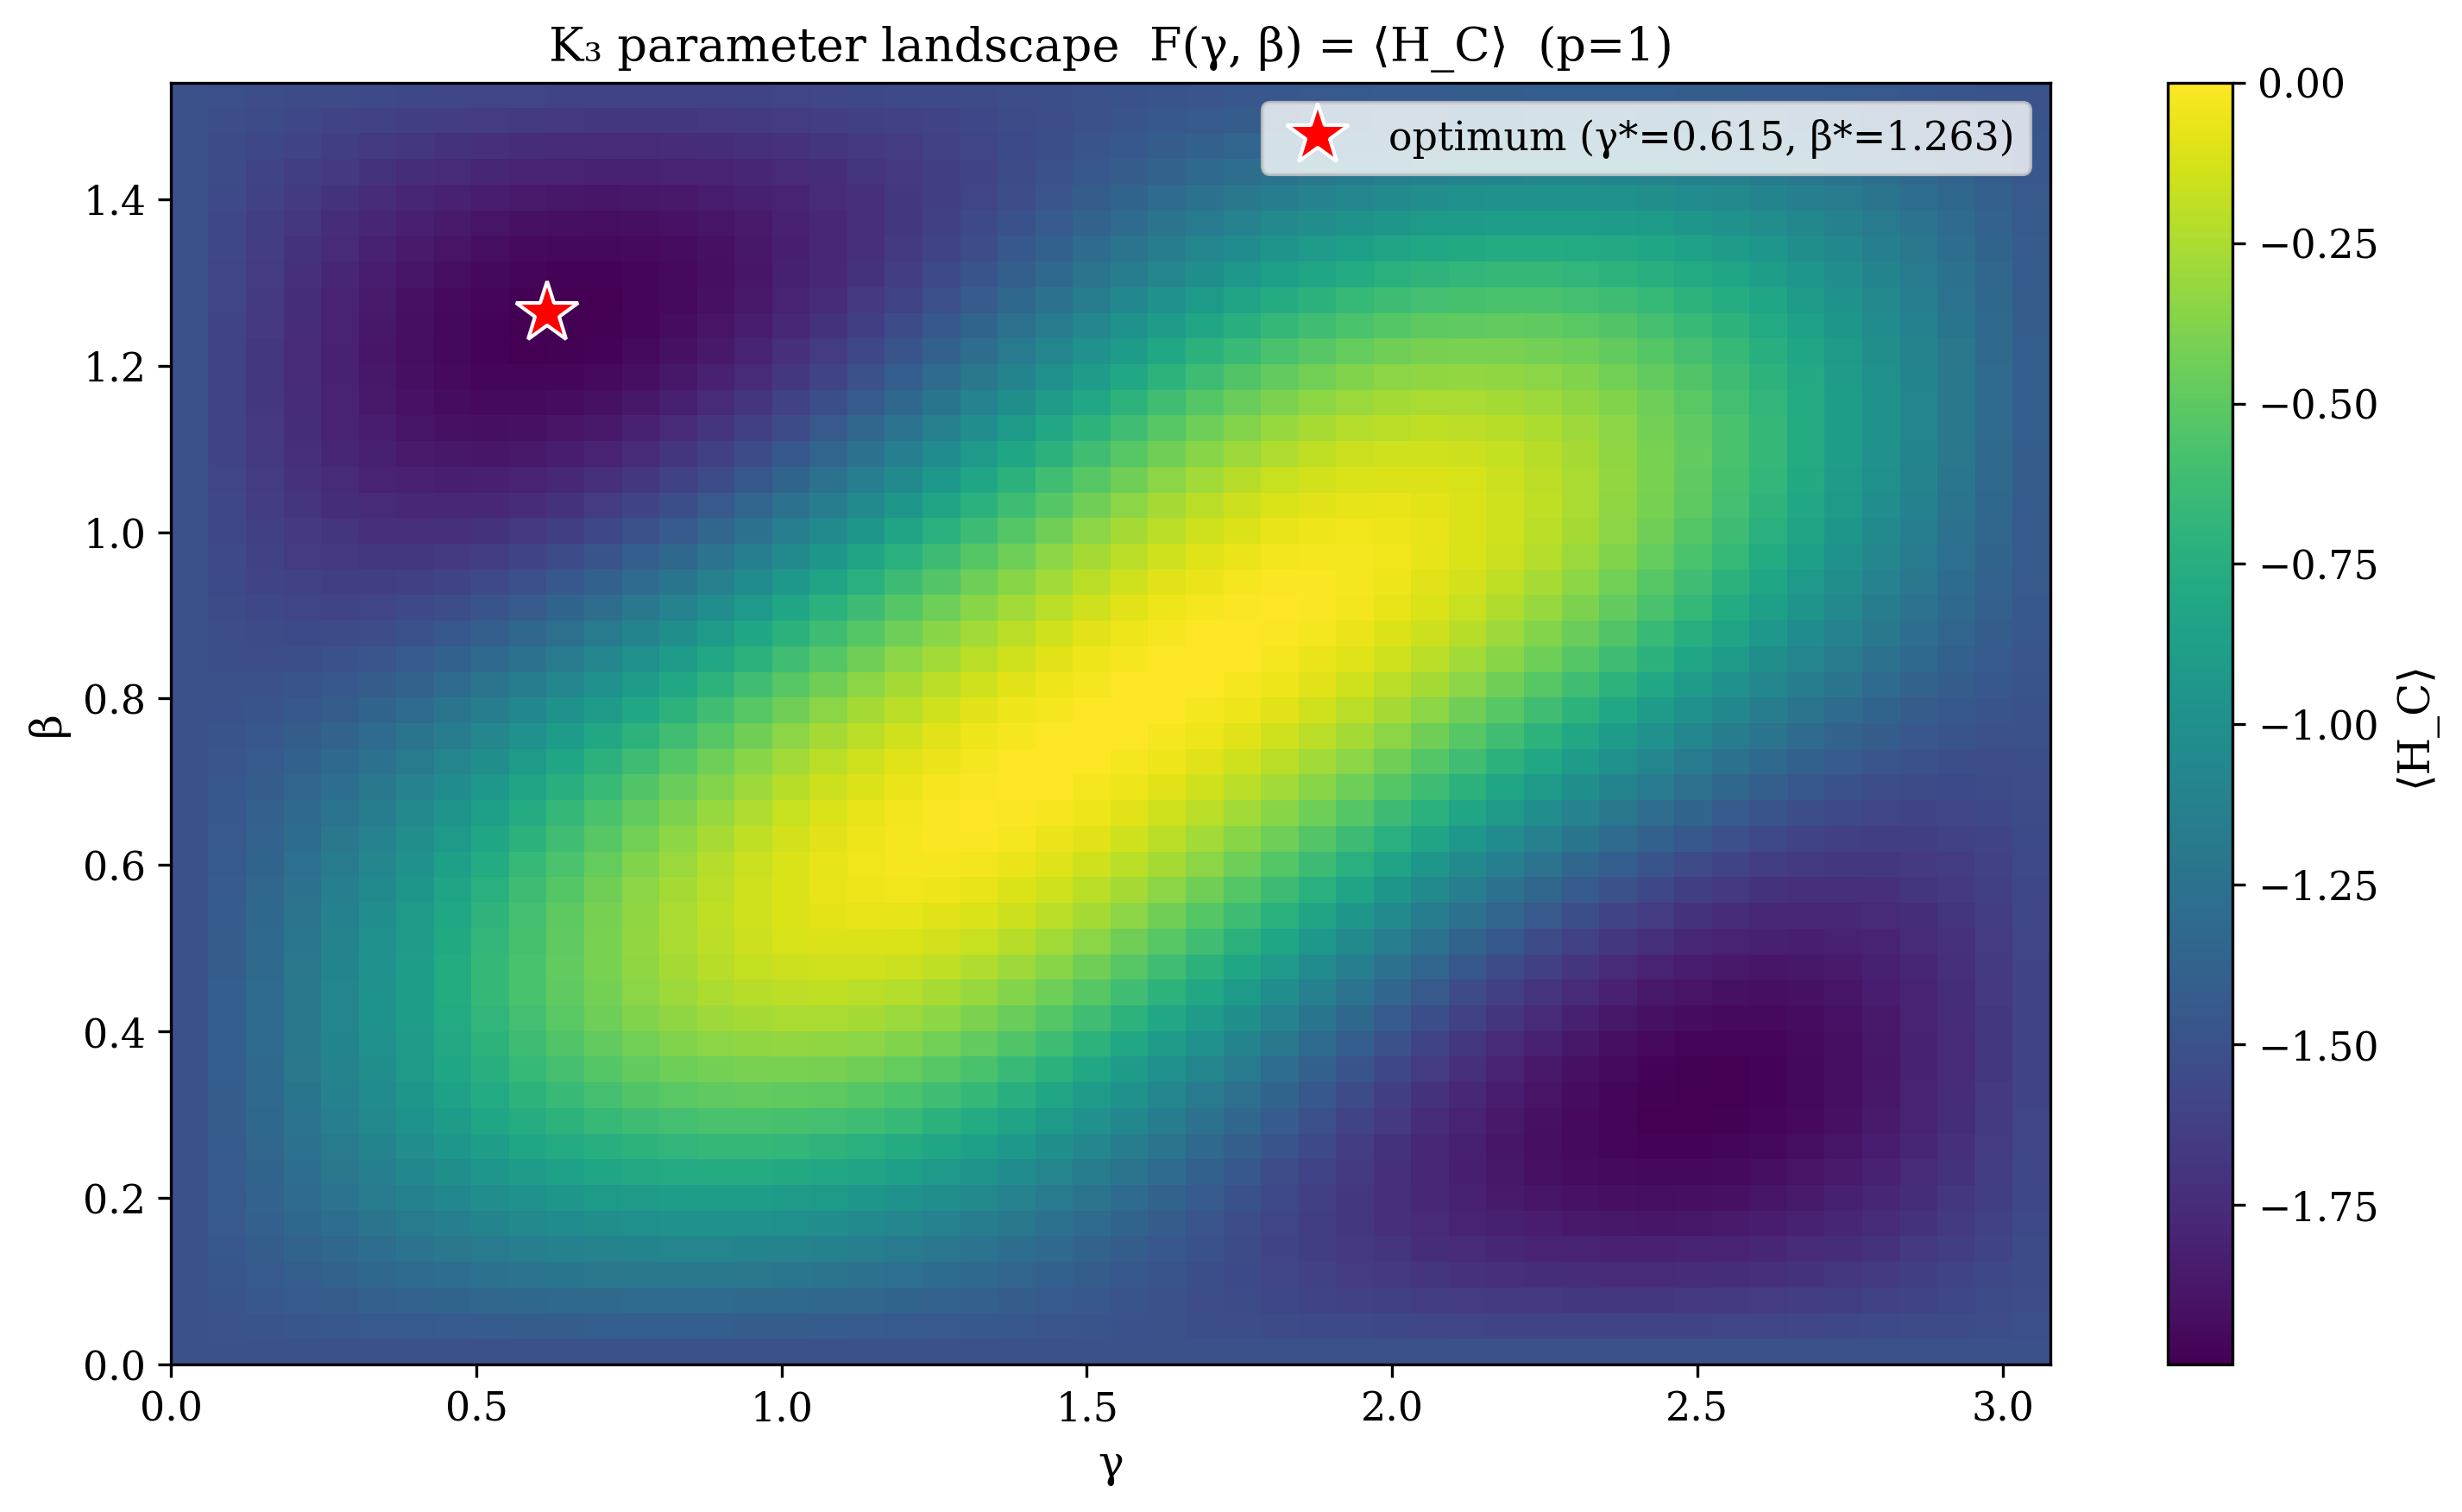
\includegraphics[width=\linewidth]{04_k3_parameter_landscape.png}
      \\[0.2em]
      {\scriptsize $F(\gamma,\beta)$ over
         $[0,\pi)\!\times\![0,\pi/2)$.  The two equivalent minima are
         related by the symmetry $F(\gamma,\beta)=F(\pi{-}\gamma, \pi/2{-}\beta)$.}
    \end{column}
  \end{columns}
  \vspace{0.4em}
  \small Both minima reach $\expect{\HC} = -2 = -\Cstar$, i.e.\ $r=1.0$ —
  \alert{$p=1$ is already sufficient for K$_3$.}
\end{frame}

% ---------------------------------------------------------------------
\begin{frame}{K$_3$ toy — convergence and measurement}
  \begin{columns}[c,onlytextwidth]
    \begin{column}{0.50\textwidth}
      \centering
      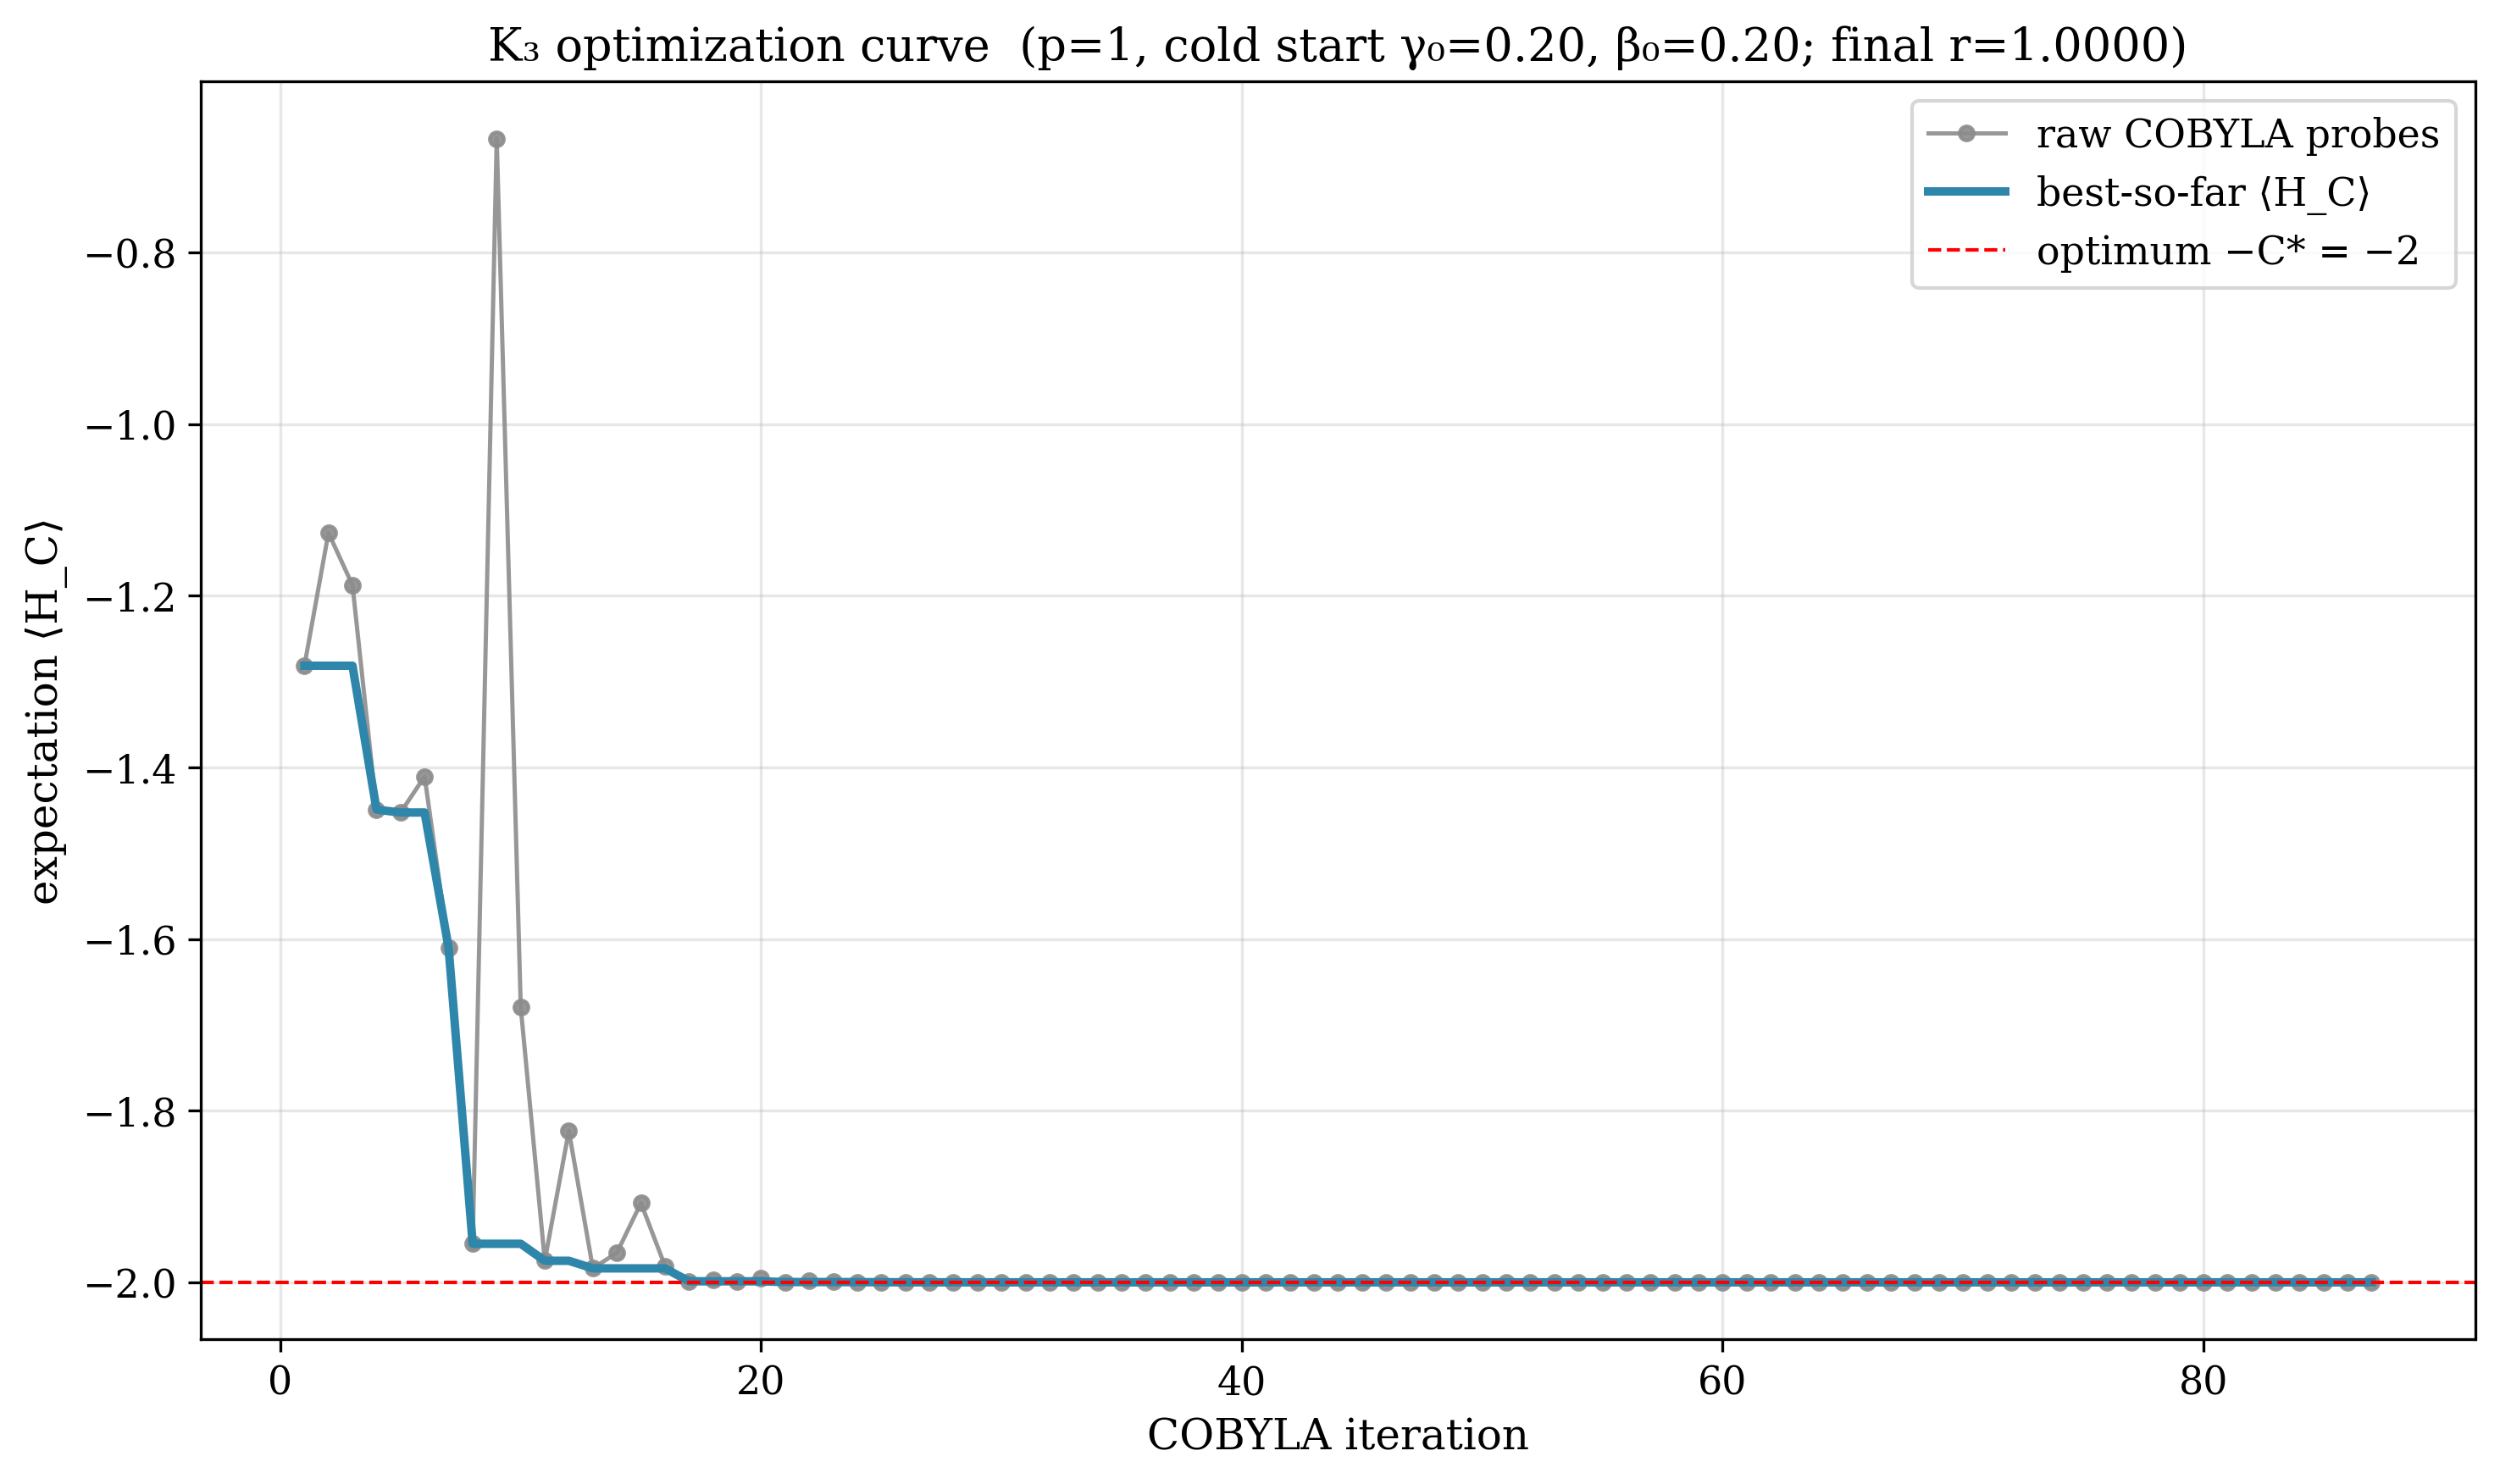
\includegraphics[width=\linewidth]{03_k3_optimization_curve.png}
      \\[0.2em]
      {\scriptsize COBYLA from a cold start
         $(\gamma_0,\beta_0)=(0.20,0.20)$; grey = raw probes, blue =
         best-so-far.}
    \end{column}
    \begin{column}{0.48\textwidth}
      \centering
      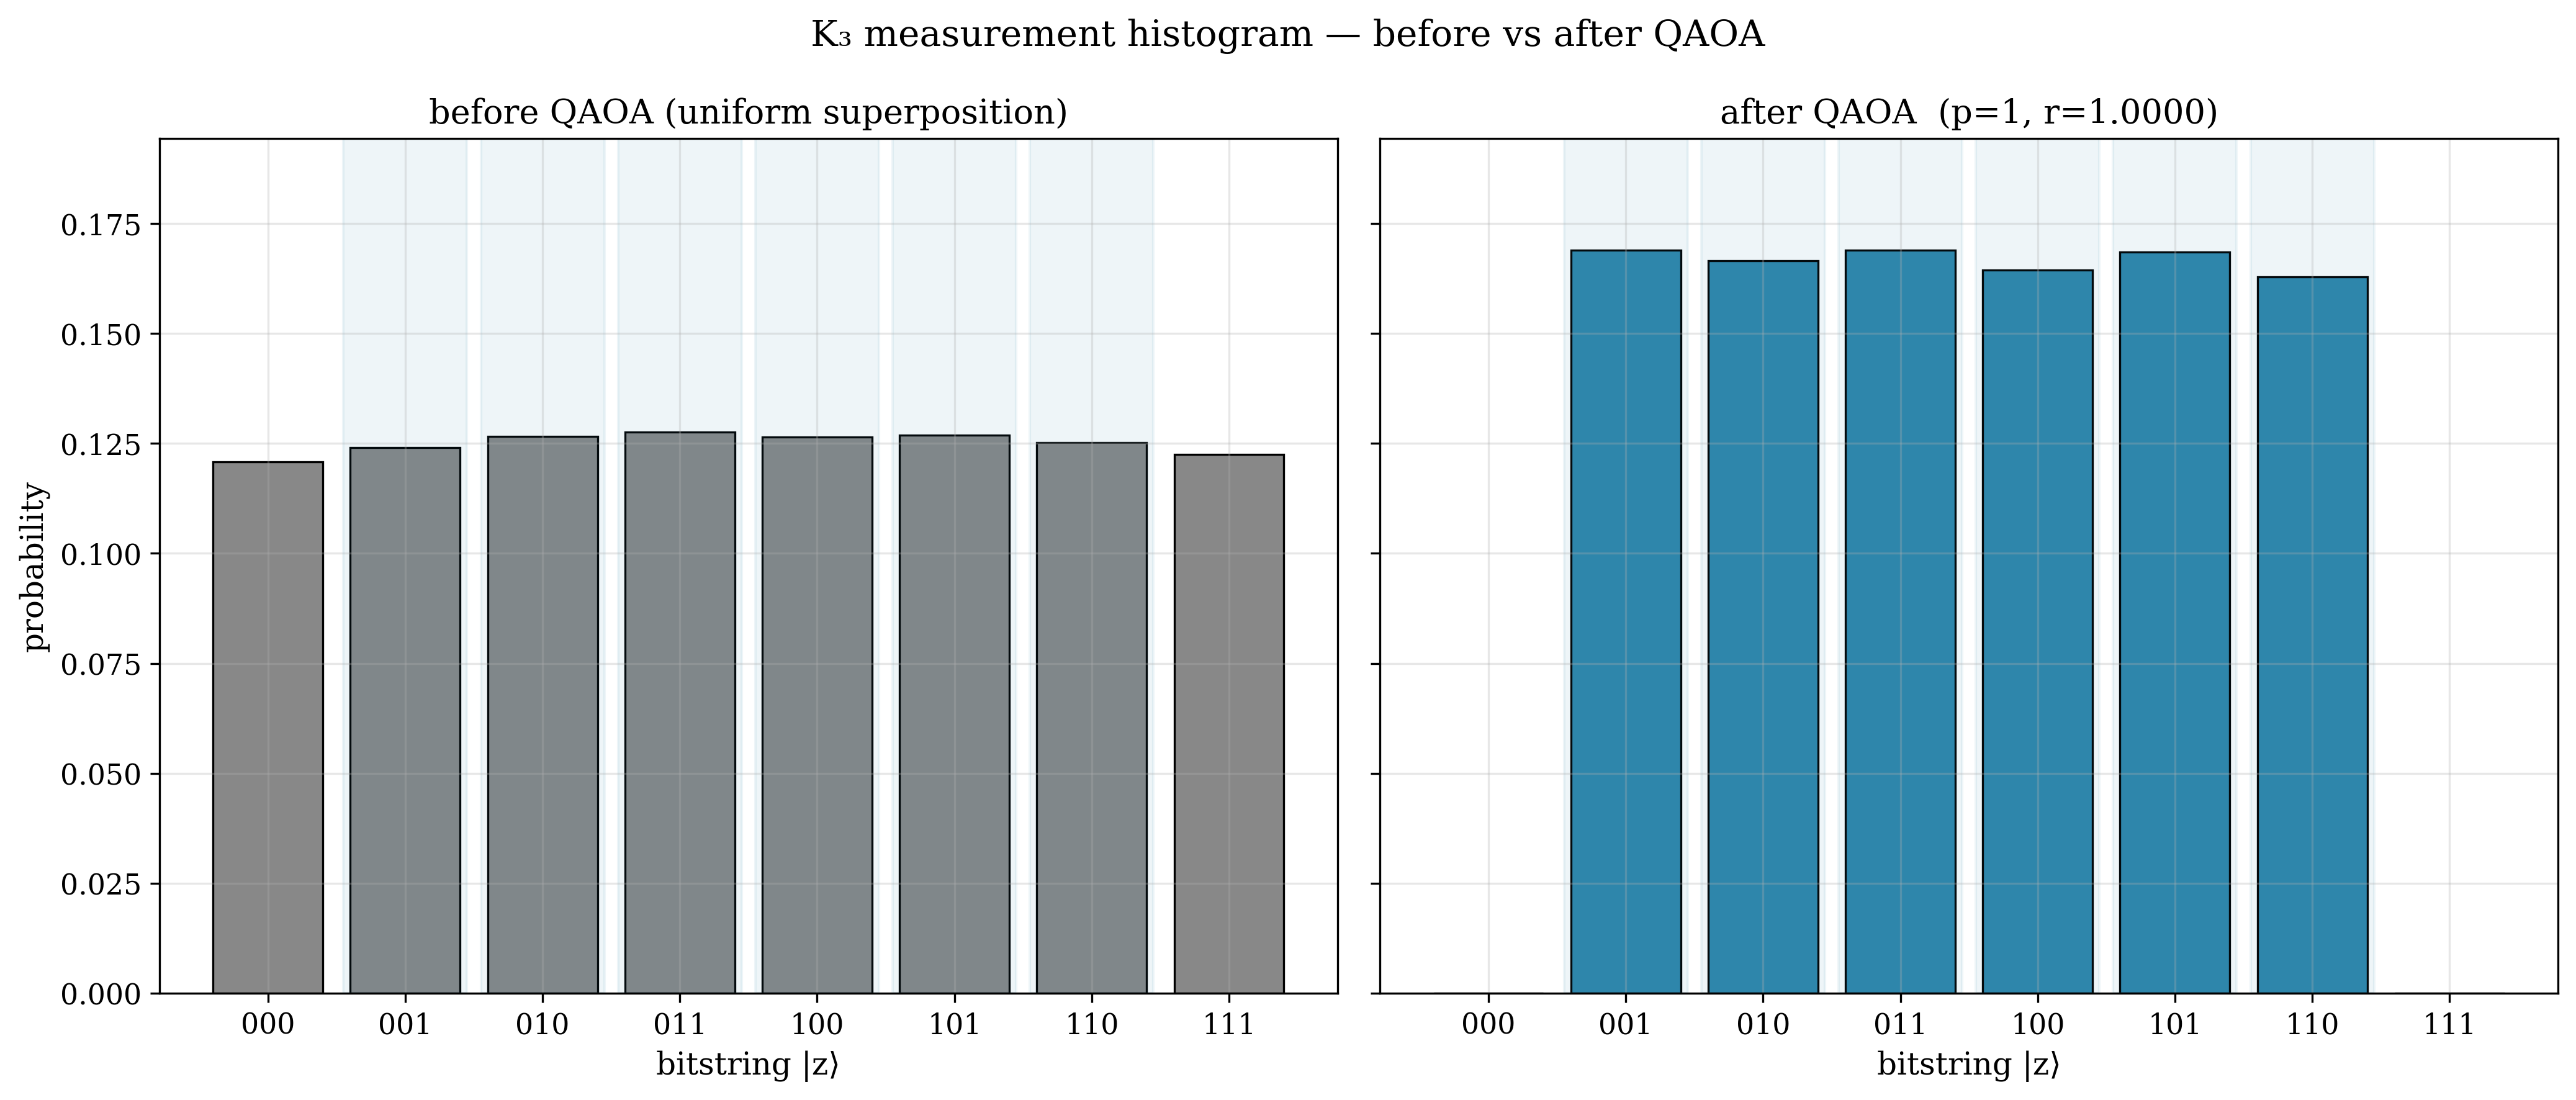
\includegraphics[width=\linewidth]{10_histogram_comparison.png}
      \\[0.2em]
      {\scriptsize $20{,}000$ shots; $\hz{000}$ and $\hz{111}$ suppressed
         to $\approx 0$, the six optimal cuts lift from $1/8$ to $1/6$.}
    \end{column}
  \end{columns}
  \vspace{0.4em}
  \small Final $r = 1.0000$ — the quantum state concentrates all
  probability on the optimal cuts.
\end{frame}

% ---------------------------------------------------------------------
\begin{frame}{Scaling study — setup}
  \begin{columns}[T,onlytextwidth]
    \begin{column}{0.55\textwidth}
      \textbf{Experiment grid}
      \begin{itemize}
        \item $N \in \{3, 4, 6, 8, 10\}$ vertices
              \begin{itemize}
                \item $N=3$: $K_3$ (triangle, 2-regular)
                \item $N \in \{4,6,8,10\}$: random 3-regular
              \end{itemize}
        \item Depth $p \in \{1, 2, 3\}$
        \item 5 seeds per $(N, p)$
        \item \textbf{Total: 75 experiments}
      \end{itemize}
      \textbf{Optimisation}
      \begin{itemize}
        \item $p=1$: $15\!\times\!15$ grid warm start
              $\to$ COBYLA refine.
        \item $p>1$: freeze prior layers, $10\!\times\!10$ mini-grid on
              new $(\gamma_q, \beta_q)$ $\to$ joint COBYLA.
      \end{itemize}
    \end{column}
    \begin{column}{0.42\textwidth}
      \centering
      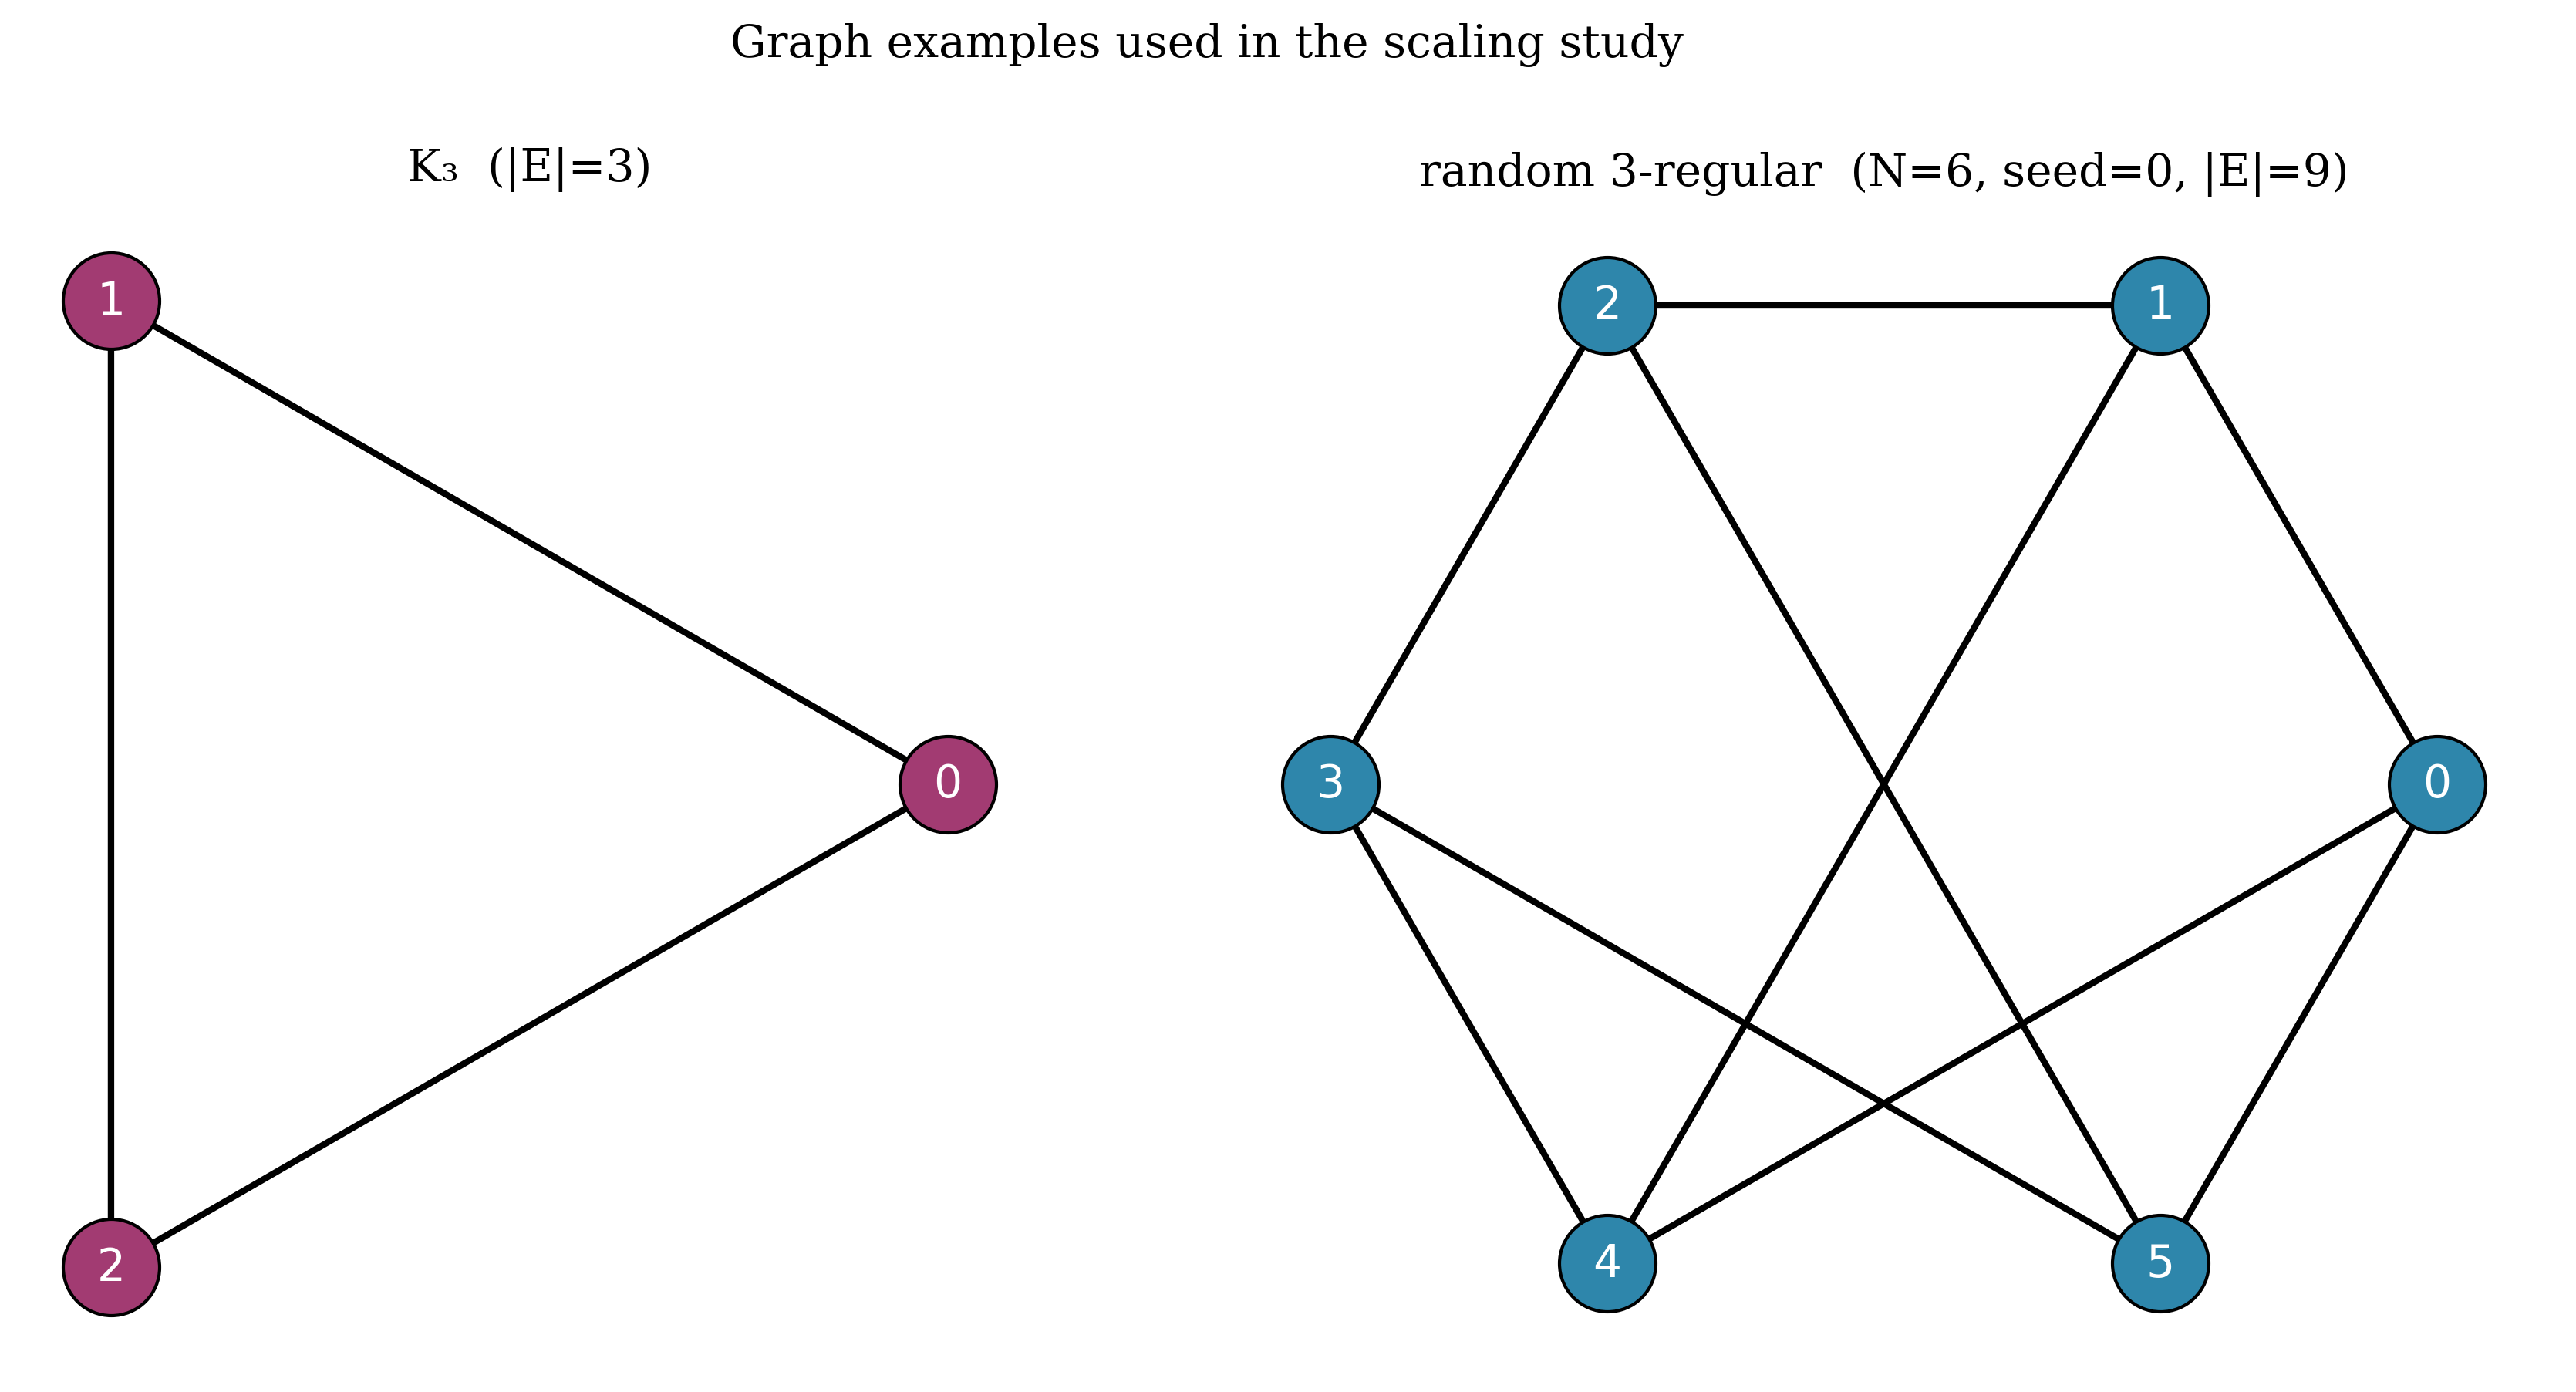
\includegraphics[width=\linewidth]{09_graph_examples.png}
      \\[0.4em]
      \footnotesize
      \textbf{Metrics collected per run:}\\
      $r$ (exact via Statevector), CNOT count, total gate count,
      circuit depth (post-transpile), COBYLA iterations, wall time.
    \end{column}
  \end{columns}
\end{frame}

% ---------------------------------------------------------------------
\begin{frame}{Scaling results — approximation ratio vs $N$}
  \begin{columns}[c,onlytextwidth]
    \begin{column}{0.58\textwidth}
      \centering
      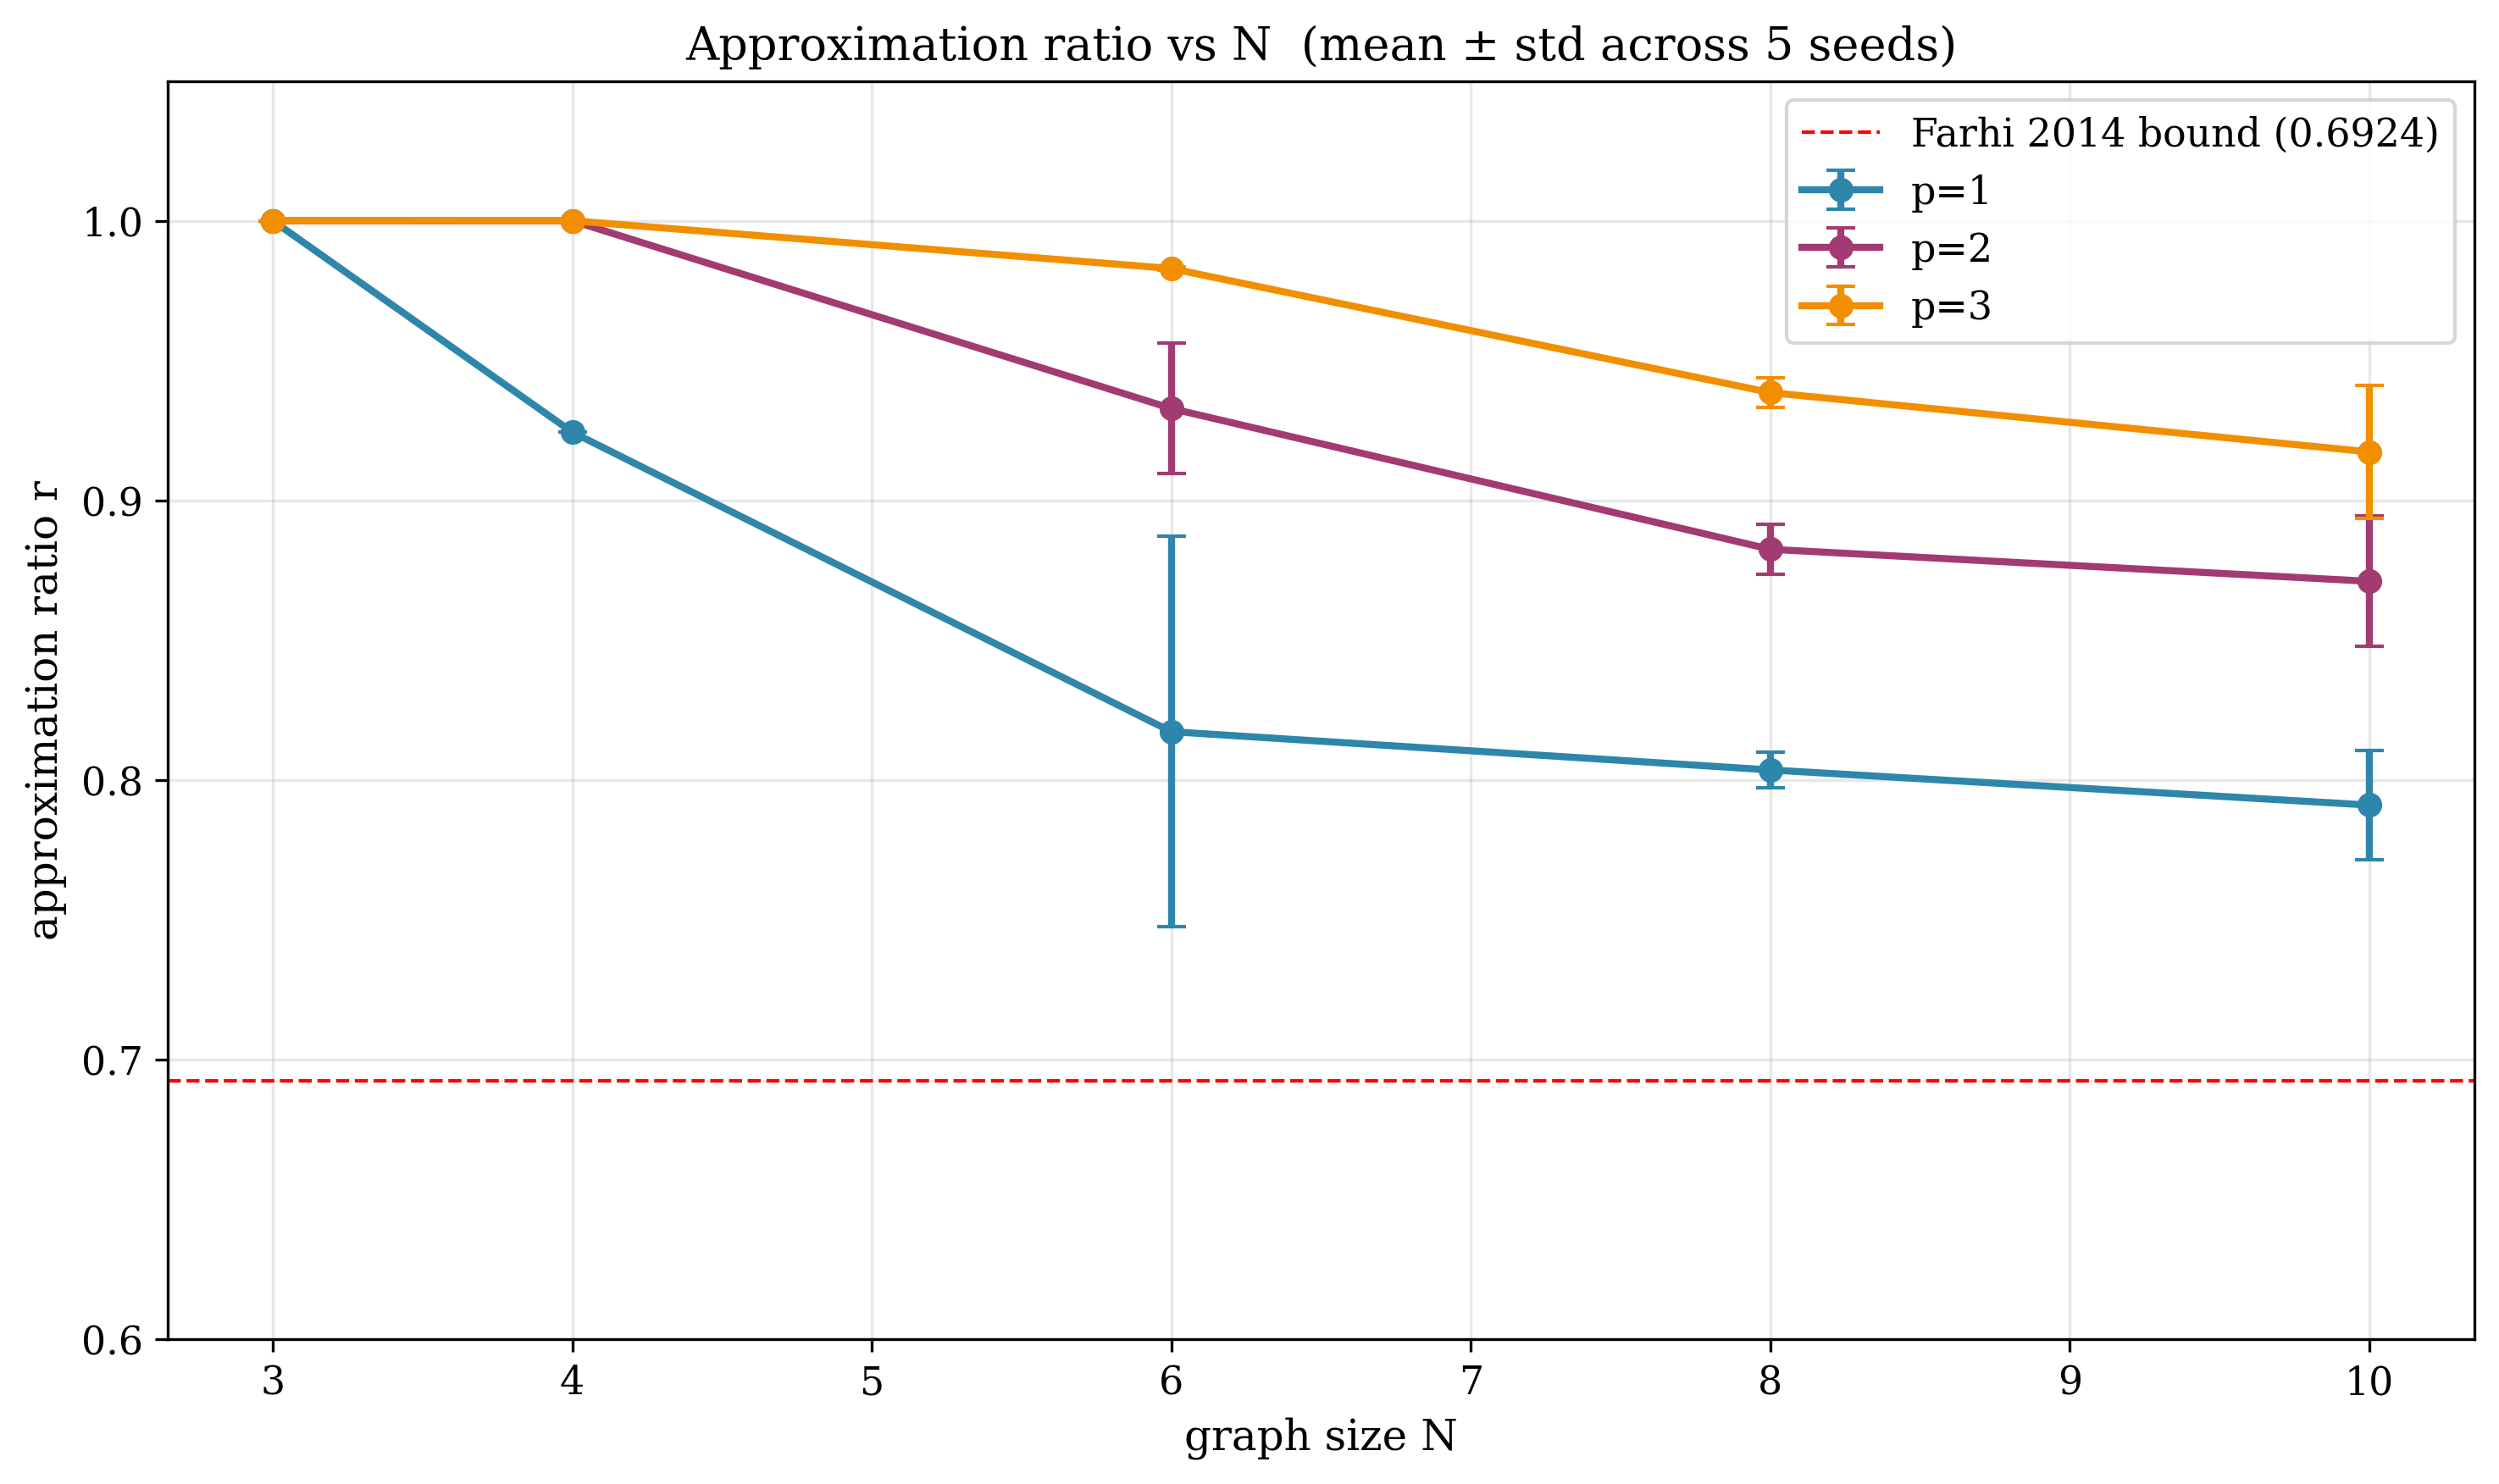
\includegraphics[width=\linewidth]{05_approximation_ratio_vs_n.png}
    \end{column}
    \begin{column}{0.40\textwidth}
      \scriptsize
      \begin{itemize}\setlength\itemsep{0.25em}
        \item All 75 runs clear the Farhi 2014 bound
              $r\ge 0.6924$ ($p=1$, 3-regular).
        \item Tightest margin: $N=6$ seed $1$, $r=0.6925$.
        \item $N=4$: all 3-regular graphs are $K_4$
              — \emph{zero} seed variance.
        \item $N=6$: widest variance, diverse 3-regular topology
              with varying QAOA hardness.
        \item $N\geq 8$: \alert{parameter concentration}
              (Brandão et al.\ 2018; Blekos et al.\ 2024)
              narrows the variance — seeds converge to similar optima.
        \item Degradation with $N$ at fixed $p$: more edges,
              same 2-parameter-per-layer ansatz.
      \end{itemize}
    \end{column}
  \end{columns}
\end{frame}

% ---------------------------------------------------------------------
\begin{frame}{Scaling results — gate cost vs $N$}
  \begin{columns}[c,onlytextwidth]
    \begin{column}{0.58\textwidth}
      \centering
      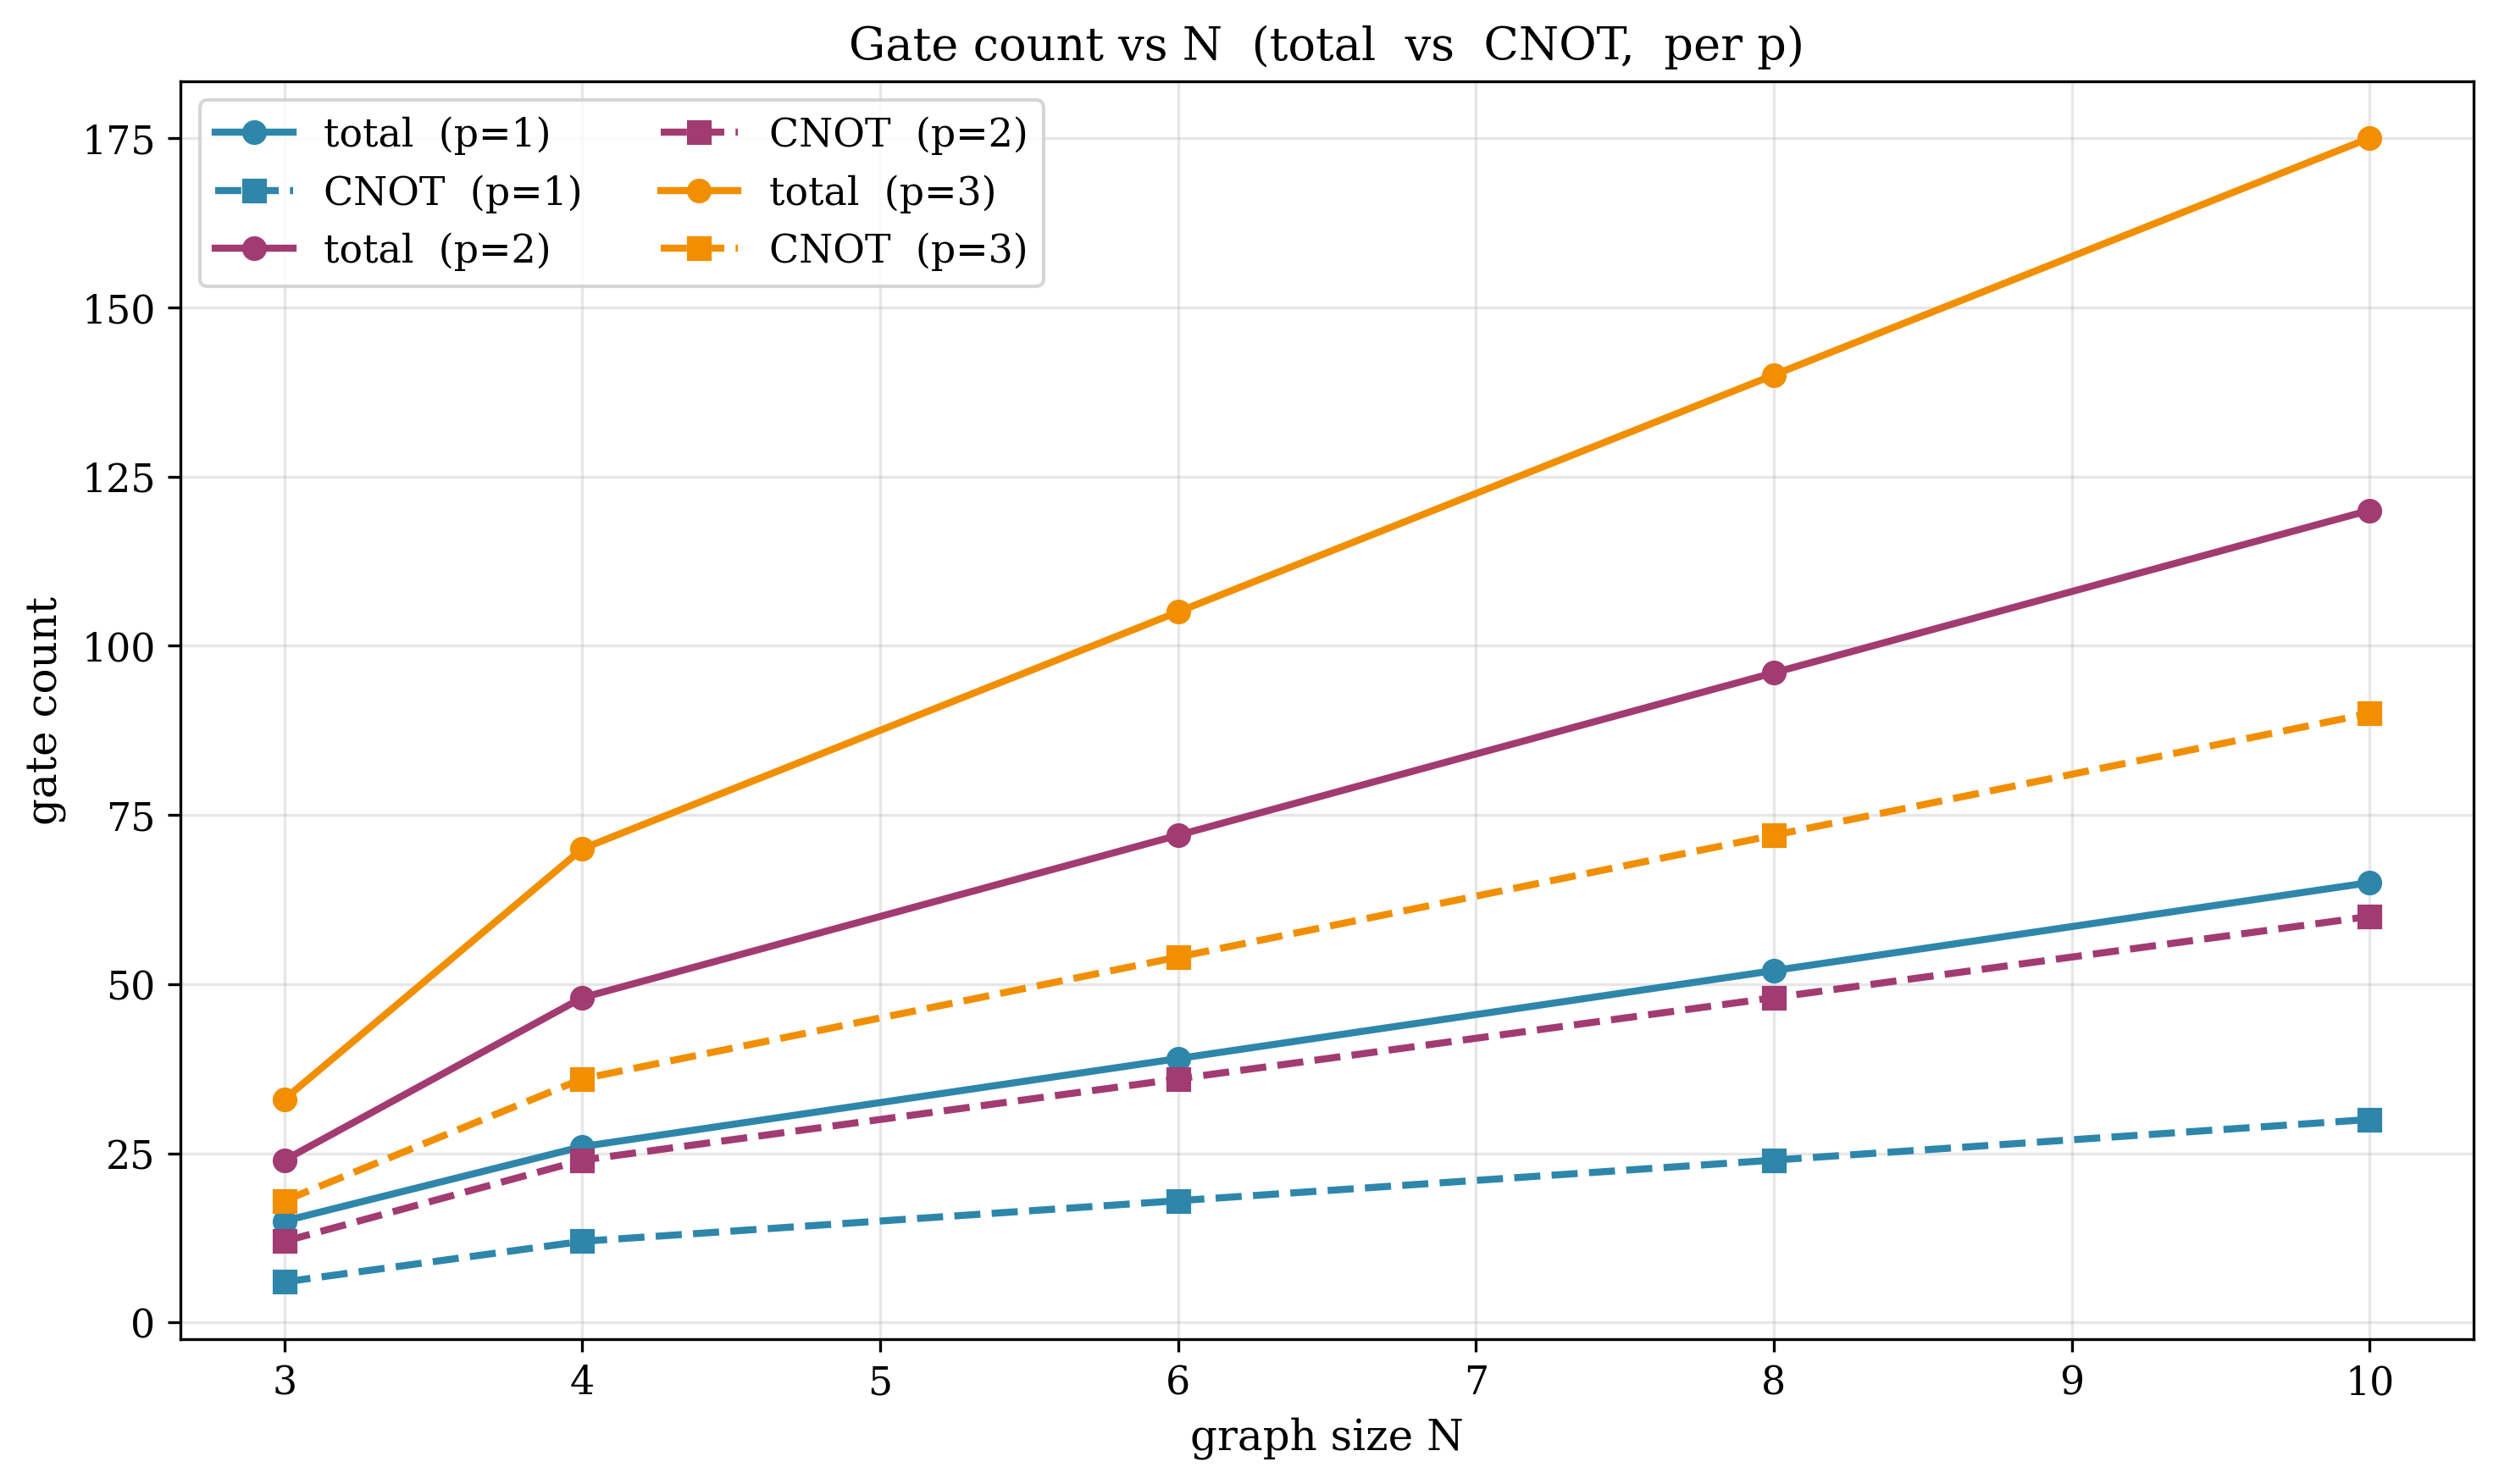
\includegraphics[width=\linewidth]{06_gate_count_vs_n.png}
    \end{column}
    \begin{column}{0.40\textwidth}
      \small
      Per layer on a 3-regular graph ($|E| = 3N/2$):
      \[
        2|E|\;\text{CX} \;+\; |E|\;R_z \;+\; N\;R_x
      \]
      plus an initial $N\,H$.  CNOTs scale \alert{linearly} in $N$,
      yielding $3N\,p$ two-qubit gates at depth $p$.
      \vspace{0.5em}

      For $N=10,\;p=3$: \textbf{90 CNOTs}, total depth $66$
      after transpile to $\{cx, rz, rx, h\}$ — comfortably within
      current NISQ coherence budgets.
      \vspace{0.3em}

      \alert{Depth scales sub-linearly:} parallelisable CNOT scheduling
      on sparse 3-regular graphs keeps depth below the raw CNOT count
      ($66 < 90$ at $N=10, p=3$).
    \end{column}
  \end{columns}
\end{frame}

% ---------------------------------------------------------------------
\begin{frame}{Depth frontier — $r$ vs $p$}
  \begin{columns}[c,onlytextwidth]
    \begin{column}{0.58\textwidth}
      \centering
      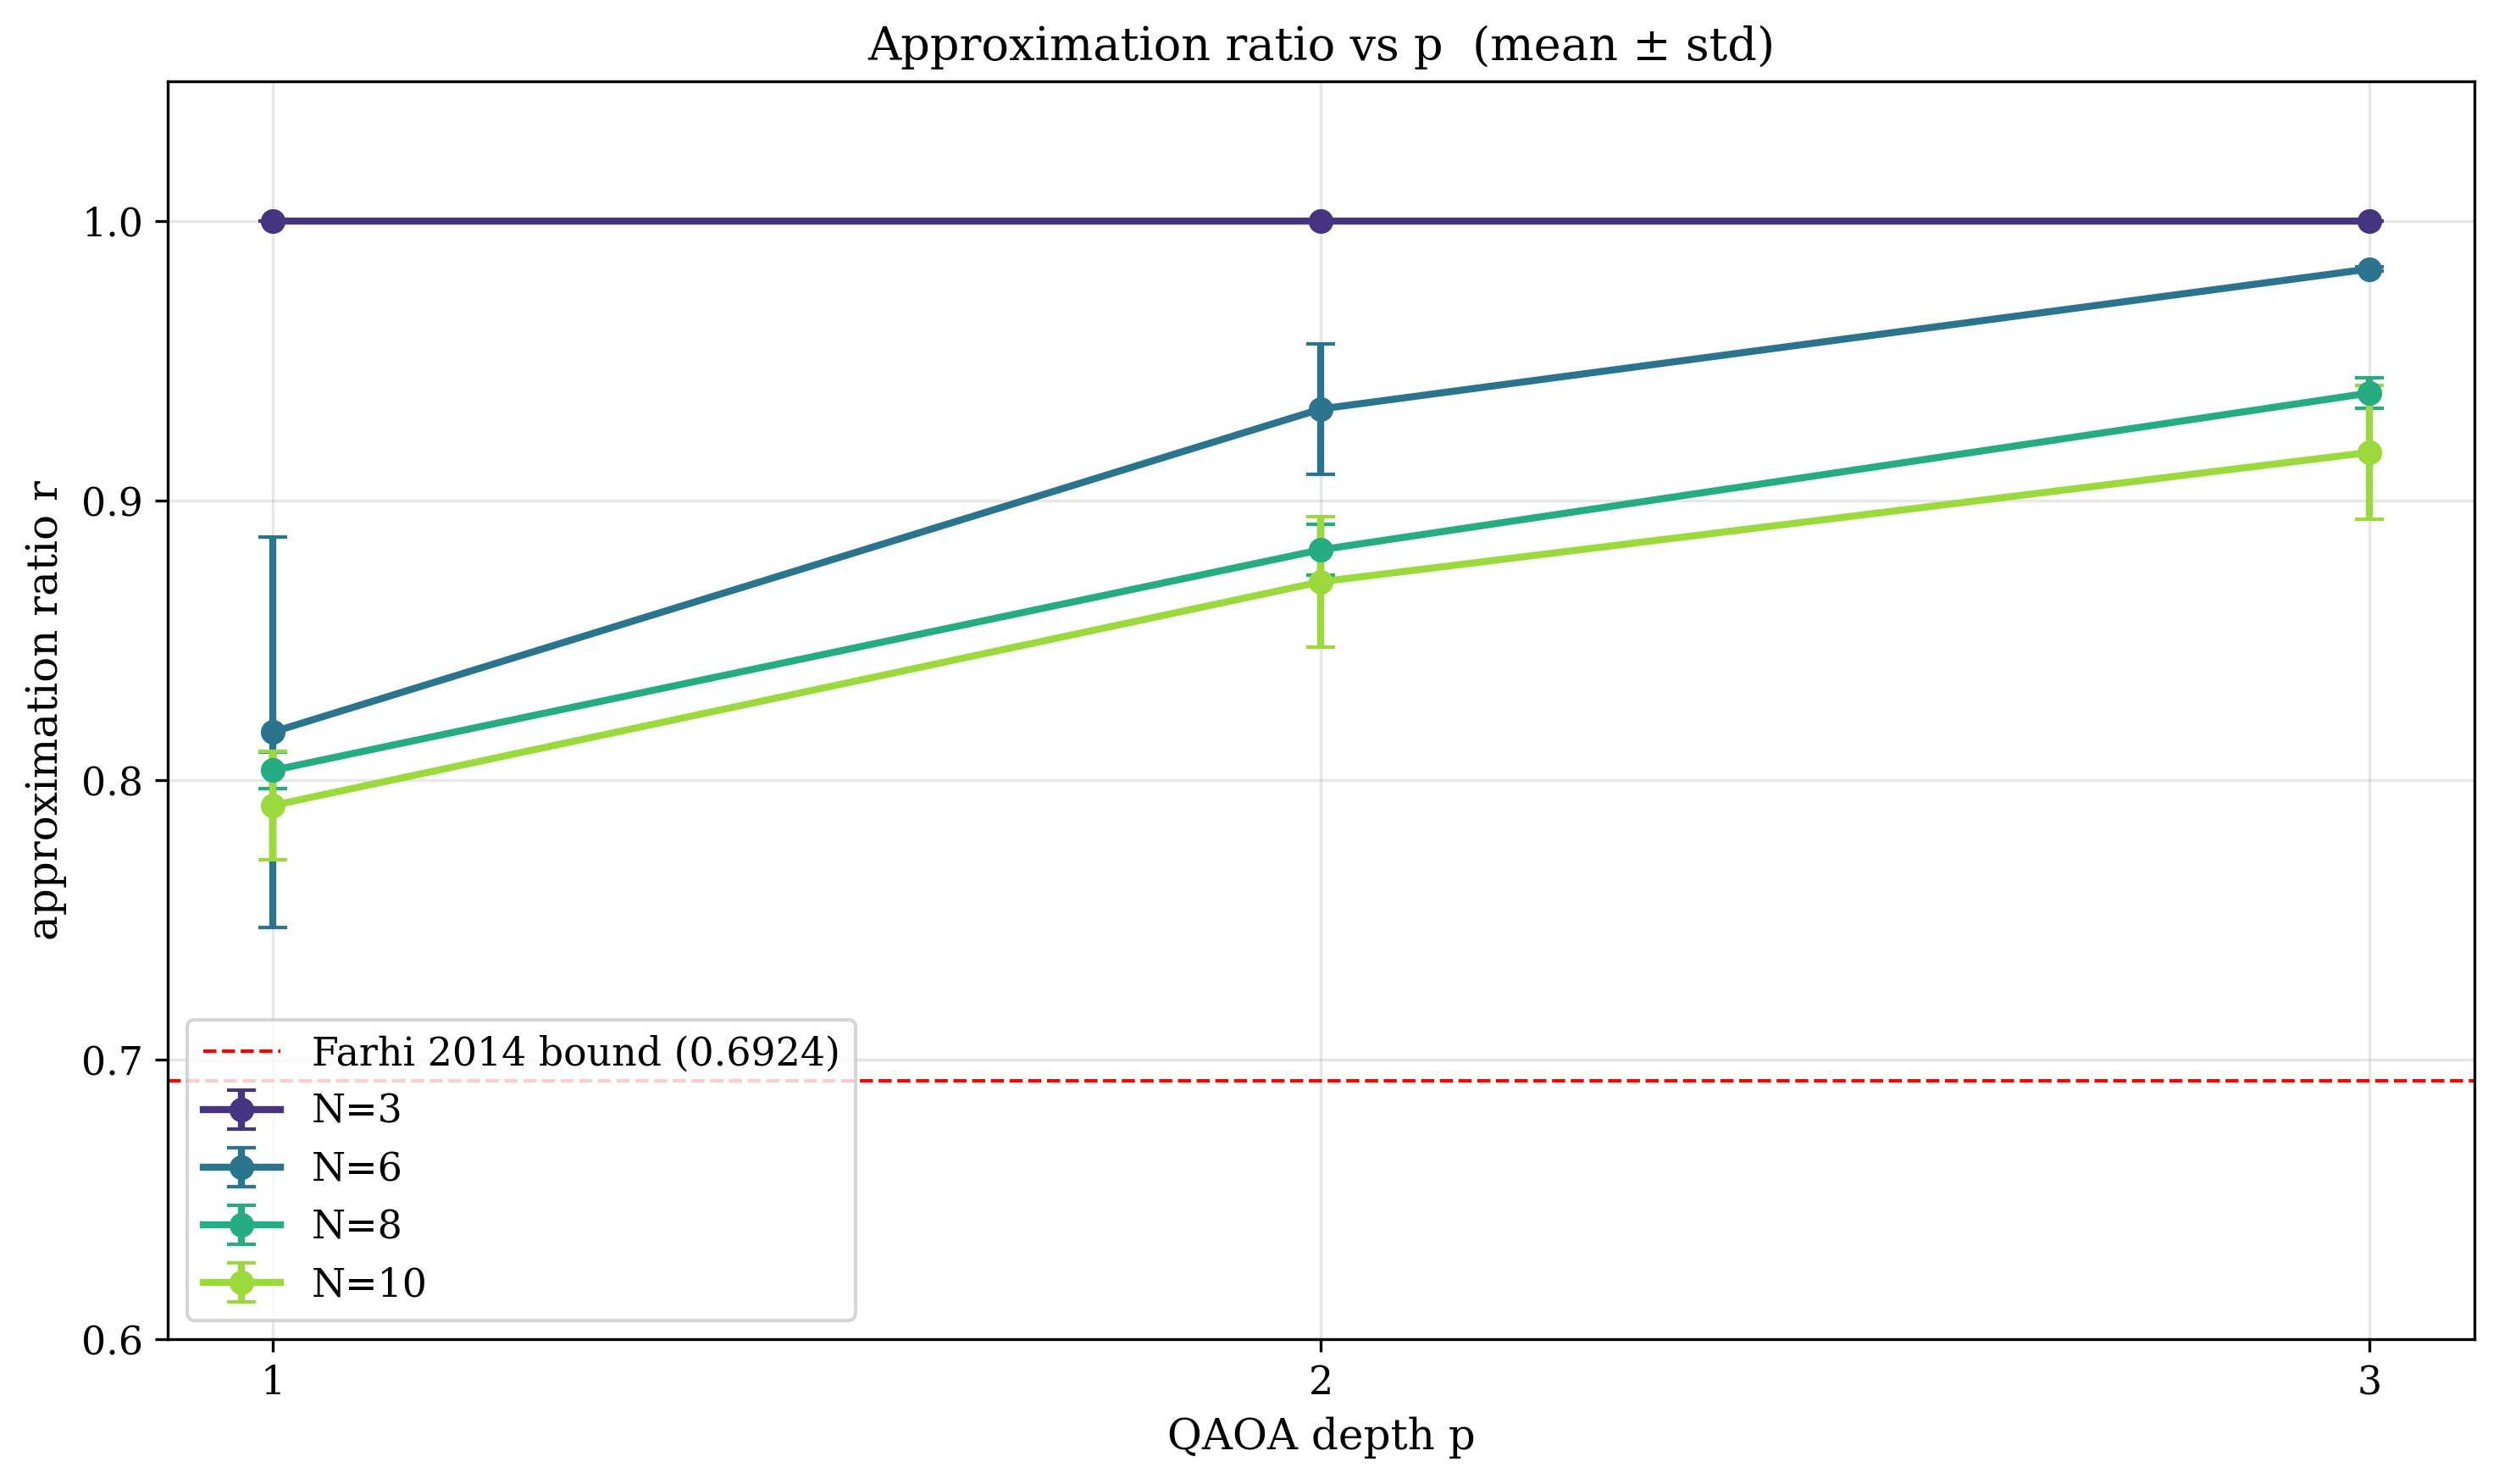
\includegraphics[width=\linewidth]{08_approximation_ratio_vs_p.png}
    \end{column}
    \begin{column}{0.40\textwidth}
      \small
      Deeper ansätze monotonically close the approximation gap:
      monotonicity holds on \textbf{all 25} $(N,\text{seed})$ pairs,
      zero violations.
      \vspace{0.4em}
      \begin{itemize}
        \item $N=3$ saturates at $p=1$.
        \item $N=10,\,p=3$: $r = 0.917 \pm 0.024$.
        \item Beats Goemans–Williamson ($0.878$) already at
              $p=2$ for $N \le 6$.
      \end{itemize}
      \vspace{0.3em}
      \emph{Trade-off:} each added layer costs another $2|E|$ CNOTs
      and $\propto$\,COBYLA wall time.
    \end{column}
  \end{columns}
\end{frame}

% ---------------------------------------------------------------------
\begin{frame}{Conclusions}
  \begin{itemize}
    \item \textbf{Validated QAOA} on 75 MaxCut instances spanning
          $N \in \{3,4,6,8,10\}$, $p \in \{1,2,3\}$, 5 seeds each.
    \item \textbf{Theoretical lower bound respected:} every $p=1$ run
          on 3-regular graphs meets $r \ge 0.6924$ (Farhi 2014).
    \item \textbf{Monotonicity} $r(p{=}1) \le r(p{=}2) \le r(p{=}3)$
          holds on every $(N, \text{seed})$ pair.
    \item \textbf{Hardware-friendly scaling:} $3Np$ CNOTs on
          3-regular graphs, linear in $N$.
    \item \textbf{Best result:} $N=10,\ p=3 \Rightarrow r = 0.917$,
          beating the classical Goemans–Williamson benchmark.
    \item The $p\to\infty$ optimality limit is theoretical;
          in the NISQ budget $p\in\{1,2,3\}$ already delivers
          $r \geq 0.87$ on all tested instances.
  \end{itemize}
  \vspace{0.8em}
  \begin{center}
    \alert{Take-away.}\ Even at $p=3$ QAOA is a credible candidate
    for near-term MaxCut on sparse graphs, with predictable
    gate and depth budgets.
  \end{center}
\end{frame}

% ---------------------------------------------------------------------
\begin{frame}{References}
  \footnotesize
  \begin{thebibliography}{9}
    \bibitem{blekos2024}
      Blekos, K., Brand, D., Ceschini, A., Chou, C.-H., Li, R.-H.,
      Pandya, K., \& Summer, A. (2024).
      \emph{A review on Quantum Approximate Optimization Algorithm
      and its variants}.
      Physics Reports, 1068, 1--66.
    \bibitem{farhi2014}
      Farhi, E., Goldstone, J., \& Gutmann, S. (2014).
      \emph{A Quantum Approximate Optimization Algorithm}.
      arXiv:1411.4028.
    \bibitem{gw1995}
      Goemans, M.~X., \& Williamson, D.~P. (1995).
      \emph{Improved approximation algorithms for maximum cut and
      satisfiability problems using semidefinite programming}.
      Journal of the ACM, 42(6), 1115--1145.
    \bibitem{preskill2018}
      Preskill, J. (2018).
      \emph{Quantum computing in the NISQ era and beyond}.
      Quantum, 2, 79.
    \bibitem{wong2022}
      Wong, T.~G. (2022). \emph{Introduction to Classical and Quantum
      Computing}. Rooted Grove.
  \end{thebibliography}
  \vfill
  \scriptsize\color{gray}
  Individual project (no co-authors).\\
  Source code, data, and figures:
  \href{https://github.com/ozgunyurutken/qaoa-project}%
       {\color{qaoablue}\texttt{github.com/ozgunyurutken/qaoa-project}}
\end{frame}

\end{document}
